\chapter{离散动力系统}
\label{chap:discrete-dynamical-systems}
\label{chap:action-and-state}
\label{chap:dynamical-systems-and-state-estimation}

每隔一分钟读一次房间与室外的温差，再给出这一分钟的加热量，下一次读数是多少？最简单的模型说：温差每分钟保留八成，再加上这一分钟的加热，即$x_{n+1}=0.8x_n+u_n$。从$x_0=0$出发、每分钟加热$0.4$，读数依次是$0.4$、$0.72$、$0.976$……一张纸、一支笔就能把它算下去。真正的问题在“算下去”之后：这串数最后停在哪里？如果起点测错了一点，或者某几分钟多加了一点热，偏差会消失、停留还是放大？如果更新规则不是线性的，长期结果还会像这里一样简单吗？我们手里的数字是计算机算出来的，舍入误差又会把轨迹带到哪里？

这些问题有一个共同的对象：一条由“当前状态加上一步更新规则”逐步生成的状态序列。本章把它作为\term{离散动力系统}（discrete dynamical system）来研究。“离散”只指时间按步编号；状态可以取实数或向量，更新可以是线性的也可以是非线性的。梯度下降的迭代、带动量的优化器、循环网络与线性状态空间模型中的隐状态更新、牛顿法的求根迭代，都是这类对象。

第~\ref{sec:dds-state-updates}节先固定比较的口径：状态应当保存什么，更新何时在每一步都有定义，多步轨迹怎样由映射复合得到，以及历史作用如何被压缩进有限个坐标。第~\ref{sec:dds-linear-recurrences}节处理线性和仿射更新，这时轨迹可以显式写出：初态的作用由矩阵幂传播，每一步的输入按“注入时刻、剩余步数”累计；时变系数需要按时间排序的矩阵乘积，而结合律又允许把串行递推改写为并行扫描。

有了显式解，第~\ref{sec:dynamical-stability-sensitivity}节才去问轨迹是否会停在平衡点或周期轨道附近。我们先区分“偏差始终小”“偏差最终消失”“偏差按几何速率消失”三种要求，再给出三类判据：线性系统看谱半径，非线性系统在平衡点处线性化，线性化不够用时寻找每步下降的Lyapunov函数。第~\ref{sec:dds-nonlinear-long-term}节离开单个平衡点，研究不收敛轨道的极限集合、参数变化引起的分岔，以及近邻轨道指数分离带来的有限精度问题。第~\ref{sec:dds-error-propagation}节把这些认识落到计算上：给定一个离散模型，舍入、残差、输入偏差和模型误差怎样沿轨迹累计。

本章把输入当作事先给定的序列；怎样根据观测去选择输入属于控制问题。连续时间的状态方程在第~\ref{chap:ordinary-differential-equations}章重新建立，随机噪声驱动的递推则在第~\ref{chap:discrete-time-stochastic-processes}章展开。

% 第1章第1节：状态更新与轨迹（递推关系与状态选择；迭代、轨道与不变集合；历史累计与状态扩充）。

\section{状态更新与轨迹}
\label{sec:dds-state-updates}

本节建立全章共用的对象。一条轨迹由四样东西决定：允许出现的状态，按步编号的时间，事先给定的外部输入，以及把当前状态和当前输入变成下一状态的更新规则。把它们分开写清，后面讨论求解、稳定和误差时才知道比较的是什么、哪些量固定不变。

\subsection{递推关系与状态选择}
\label{sec:dds-recurrence-state}

\paragraph{一分钟一步的温度}
回到章首的房间。环境温度固定，$x_n$表示第$n$分钟时房间相对环境的温差，$u_n$表示第$n$分钟内的加热量。模型
\begin{equation}
  x_{n+1}=0.8x_n+u_n
  \label{eq:dds-temperature}
\end{equation}
说：不加热时，温差每分钟保留八成，其余散到环境里；加热则直接补充温差。取$x_0=0$、$u_n=0.4$，逐步代入得到
\[
  \begin{gathered}
  x_1=0.4,\quad x_2=0.72,\quad x_3=0.976,\\
  x_4=1.1808,\quad x_5=1.34464,\quad x_6\approx1.4757.
  \end{gathered}
\]
数列在增长，增量却越来越小，看上去在逼近某个值。

这个值可以从递推式本身读出。若存在不随时间改变的温差$x_*$，它必须满足$x_*=0.8x_*+0.4$，即$x_*=2$。把式~\eqref{eq:dds-temperature}两边同减$2$，
\[
  x_{n+1}-2=0.8x_n+0.4-2=0.8\,(x_n-2).
\]
所以与平衡值的偏差每一步乘以$0.8$：$x_n-2=0.8^n(x_0-2)=-2\times0.8^n$。图~\ref{fig:dds-temperature-trajectory}把三条不同起点的轨迹画在一起：无论从下方还是上方出发，它们都向$2$靠拢；换成对数纵轴后，三条偏差曲线变成斜率相同的平行直线，斜率就是$\ln0.8$。

\begin{figure}[htbp]
  \centering
  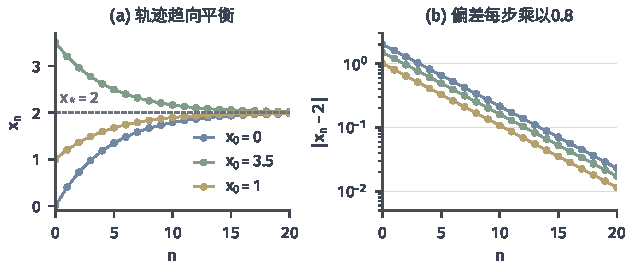
\includegraphics[width=107mm]{figures/03-optimization-evolution-and-signals/02-processes-and-trajectory-evolution/matplotlib/dds-temperature-trajectory/figure.pdf}
  \caption{温度递推$x_{n+1}=0.8x_n+0.4$的轨迹。(a)三个初值$x_0=0,\,1,\,3.5$的前$20$步，虚线为平衡温差$x_*=2$；(b)同三条轨迹的偏差$|x_n-2|$，纵轴取对数。偏差每步乘以$0.8$，在对数坐标中是斜率为$\ln0.8$的平行直线，起点只决定直线的高低。}
  \label{fig:dds-temperature-trajectory}
\end{figure}

这个小计算已经把两个量分开了。平衡位置$x_*=u/(1-0.8)$由系数和输入共同决定：把恒定加热改成$0.5$，平衡升到$2.5$。接近平衡的速度只由系数$0.8$决定：输入改变时，偏差仍然每步乘以$0.8$；系数改成$0.5$，偏差每步减半，接近得快得多。只报告“最终温度”不能说明轨迹，因为同一个终点可以由快慢完全不同的过程到达。

\paragraph{状态应当记住什么}
式~\eqref{eq:dds-temperature}之所以能一步一步算下去，是因为下一时刻的温差只依赖当前温差和当前加热量，过去更早的加热已经全部体现在$x_n$里。这个性质不是变量名称自动带来的，而是模型的假设。假如墙体也会蓄热：同样的室温下，墙体较热时房间散热慢，墙体较冷时散热快，那么只看室温就预测不了下一分钟。

设$h_n$为墙体相对环境的温差，取教学用的扩充模型
\[
  \begin{bmatrix}x_{n+1}\\h_{n+1}\end{bmatrix}
  =\begin{bmatrix}0.8&0.1\\0.1&0.9\end{bmatrix}
   \begin{bmatrix}x_n\\h_n\end{bmatrix}
  +\begin{bmatrix}0.4\\0\end{bmatrix}.
\]
两个初态都有$x_0=0$，加热量也相同，但$h_0=2$给出$x_1=0.6$，$h_0=-2$给出$x_1=0.2$。图~\ref{fig:dds-state-sufficiency}把两条轨迹继续画下去：相同的当前室温对应不同的未来。对这个模型，室温一个坐标不够，必须把$(x_n,h_n)$一起记作状态。

\begin{figure}[htbp]
  \centering
  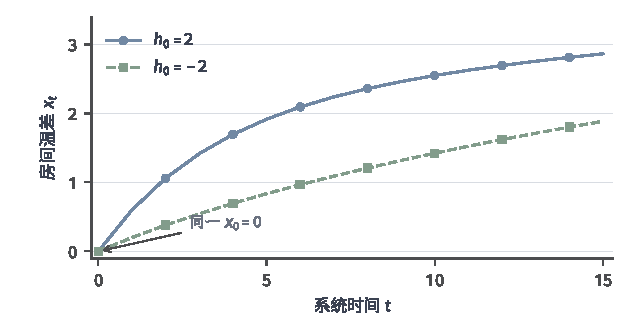
\includegraphics[width=107mm]{figures/00-shared/mathematical-preliminaries-lower/02-dynamical-systems-control-decision-and-games/matplotlib/reader-state-sufficiency/figure.pdf}
  \caption{室温单坐标遗漏墙体蓄热时的预测差异。按正文的双状态教学模型逐步计算，两条曲线的房间初始温差均为$x_0=0$，恒定加热量均为$0.4$；仅墙体初始温差$h_0$分别取$2$与$-2$。相同的当前室温对应不同的后继轨迹，说明状态要按“未来依赖什么”来选。}
  \label{fig:dds-state-sufficiency}
\end{figure}

由此可以给出本章的基本对象。选择状态的标准是：已知当前状态和当前输入，下一状态就被唯一确定，不必再回看更早的历史。

\begin{definition}[离散时间状态模型]
\label{def:dds-state-model}
设$X$为非空集合，称为\term{状态空间}（state space）；$U$为非空集合，称为输入集合。对每个$n\in\mathbb N$给定映射$F_n:X\times U\to X$。对初值$x_0\in X$与输入序列$(u_n)_{n\geq0}\subseteq U$，递推
\begin{equation}
  x_{n+1}=F_n(x_n,u_n),\qquad n=0,1,2,\ldots
  \label{eq:dds-state-model}
\end{equation}
唯一确定序列$(x_n)_{n\geq0}$，称为从$x_0$出发、受输入$(u_n)$驱动的\term{轨迹}（trajectory）。$x_n$称为时刻$n$的\term{状态}（state）。
\end{definition}

定义要求$F_n$的值仍落在$X$中，这是“每一步都有定义”的保证：只要$x_n\in X$，$x_{n+1}$就有意义，归纳下去整条轨迹都有意义。实际建模时，更新公式往往只在某个区域内有意义，比如要开平方根或取对数；这时必须把$X$取成公式能映回自身的集合，或者逐步检查轨迹没有离开公式的定义域。第~\ref{sec:dds-orbits-invariant}小节会用不变区间系统地处理这件事。

\paragraph{高阶递推改写为一阶向量递推}
状态选择的另一种常见情形来自高阶递推。用带动量的梯度下降最小化$f(\theta)=\theta^2/2$，步长$\eta$、动量系数$\beta$时，参数按
\[
  \theta_{n+1}=\theta_n-\eta\theta_n+\beta(\theta_n-\theta_{n-1})
\]
更新。取$\eta=0.5$、$\beta=0.4$，得到二阶递推
\begin{equation}
  \theta_{n+1}=0.9\,\theta_n-0.4\,\theta_{n-1}.
  \label{eq:dds-heavy-ball}
\end{equation}
只知道$\theta_n$不能算出$\theta_{n+1}$：$\theta_n=1$时，$\theta_{n-1}=1$给出$0.5$，$\theta_{n-1}=0$给出$0.9$。动量项记住了“上一步走了多远”，这正是当前参数值没有包含的信息。

办法是把需要的历史并进状态。令$\bm z_n=(\theta_n,\theta_{n-1})^{\top}\in\mathbb R^2$，则
\begin{equation}
  \bm z_{n+1}=\begin{bmatrix}\theta_{n+1}\\ \theta_n\end{bmatrix}
  =\begin{bmatrix}0.9&-0.4\\1&0\end{bmatrix}\bm z_n .
  \label{eq:dds-heavy-ball-state}
\end{equation}
第一行就是原递推，第二行只是把$\theta_n$抄到下一个状态的第二个位置（图~\ref{fig:dds-state-augmentation}）。初值需要两个数$(\theta_0,\theta_{-1})$，这与二阶递推需要两个初始条件一致。同样的做法适用于任意$k$阶递推$x_{n+1}=G(x_n,\ldots,x_{n-k+1},u_n)$：取最近$k$个值组成的向量为状态，状态空间变成$X^k$，更新仍是一阶的。

\begin{figure}[htbp]
  \centering
  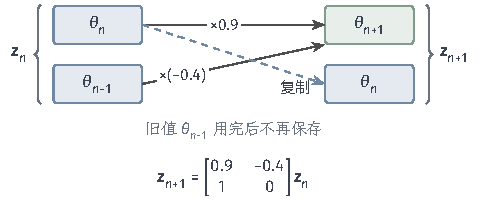
\includegraphics[width=90mm]{figures/03-optimization-evolution-and-signals/02-processes-and-trajectory-evolution/tikz/dds-state-augmentation/figure.pdf}
  \caption{二阶递推$\theta_{n+1}=0.9\theta_n-0.4\theta_{n-1}$的状态扩充。状态$\bm z_n$同时保存$\theta_n$与$\theta_{n-1}$；一步更新用两者算出$\theta_{n+1}$，并把$\theta_n$复制到新状态的第二个位置，最旧的值随之丢弃。整个操作是一次$2\times2$矩阵乘法。}
  \label{fig:dds-state-augmentation}
\end{figure}

这个例子后面还会出现：第~\ref{sec:dds-constant-coefficient}小节将看到，矩阵~\eqref{eq:dds-heavy-ball-state}有一对复特征值，所以动量迭代会一边振荡一边收敛。

\paragraph{自治、线性与时变}
有了一般形式，就可以按更新规则的结构给系统分类。若$F_n=F$不依赖$n$，且没有输入或输入恒定，系统写成$x_{n+1}=F(x_n)$，称为\term{自治}（autonomous）系统；否则称为非自治系统。给定一条输入序列后，令$F_n^{u}(x)=F_n(x,u_n)$，系统就成为只含状态的非自治递推$x_{n+1}=F_n^{u}(x_n)$。本章讨论稳定性时主要使用自治形式，恒定输入的情形通过平移平衡点化归过来。

另一种分类看$F_n$是否线性。当$X=\mathbb R^d$、$U=\mathbb R^m$时，\term{线性系统}（linear system）指
\begin{equation}
  \bm x_{n+1}=\bm A_n\bm x_n+\bm B_n\bm u_n,\qquad
  \bm A_n\in\mathbb R^{d\times d},\ \bm B_n\in\mathbb R^{d\times m},
  \label{eq:dds-linear-system}
\end{equation}
它关于状态与输入的联合变量$(\bm x,\bm u)$是线性映射。系数矩阵不随$n$变化时称为时不变或定常，否则称为时变。线性与时变是两项相互独立的性质：$x_{n+1}=0.8x_n+\sin n$是线性时变的，$x_{n+1}=x_n^2$是非线性时不变的。“离散时间”又是第三项独立的性质，它只说明时间按步编号。

线性有两个容易混淆的地方。第一，固定一条非零输入后，$\bm x\mapsto\bm A\bm x+\bm B\bm u_n$关于状态是\term{仿射映射}（affine map），不是线性映射：温度模型~\eqref{eq:dds-temperature}在$u_n=0.4$时，从$x_0=0$与$x_0=1$出发的第一步分别是$0.4$和$1.2$，而从$x_0=0+1$出发的第一步是$1.2$，不等于$0.4+1.2$。叠加原理对初值与输入一起成立，对初值单独不成立。第二，“系数乘状态”的外形不能保证线性。$x_{n+1}=(0.5+0.1x_n^2)\,x_n$看上去像系数$0.5+0.1x_n^2$乘以$x_n$，但系数本身依赖状态，把初值加倍后下一步并不加倍：$x_0=1$给出$0.6$，$x_0=2$给出$1.8$。

\subsection{迭代、轨道与不变集合}
\label{sec:dds-orbits-invariant}

\paragraph{多步映射与前向轨道}
自治系统$x_{n+1}=F(x_n)$的多步状态由映射复合给出。记$F^0=\operatorname{id}$，$F^{n}=F\circ F^{n-1}$，则$x_n=F^n(x_0)$。本章中映射的上标$F^n$一律表示$n$次复合，而不是函数值的$n$次幂；对线性映射$\bm x\mapsto\bm A\bm x$，$n$次复合恰好是矩阵幂$\bm A^n$，两种读法一致。复合满足
\[
  F^{m+n}=F^m\circ F^n,\qquad m,n\geq0,
\]
即走$m+n$步等于先走$n$步、再从到达的位置走$m$步。这条性质说明状态确实“概括了过去”：从$x_n$重新开始计算，与从$x_0$一口气算下去得到同样的未来。

非自治系统也有多步映射，只是要按时间排序：
\[
  x_n=(F_{n-1}\circ\cdots\circ F_1\circ F_0)(x_0),
\]
较晚的更新写在左边，因为它作用在较早更新的结果上。顺序不能交换：$F_0(x)=2x$、$F_1(x)=x+1$时，从$x_0=1$出发得$F_1(F_0(1))=3$，若误写成$F_0(F_1(1))$则得到$4$。

\begin{definition}[轨道与不变集合]
\label{def:dds-orbit-invariant}
设$F:X\to X$。点$x_0\in X$的\term{轨道}（orbit）指序列$(F^n(x_0))_{n\geq0}$，其取值集合$\{F^n(x_0):n\geq0\}$称为前向轨道集合。若子集$S\subseteq X$满足$F(S)\subseteq S$，称$S$为\term{正向不变集}（positively invariant set）；若$F(S)=S$，称$S$为\term{不变集}（invariant set）。
\end{definition}

正向不变集的意思是“进得来、出不去”：若$x_0\in S$，归纳可知全部$x_n\in S$。不变集还多要求一件事：$S$中每一点都有$S$中的前像，因而可以在$S$内往过去追溯。区分二者在第~\ref{sec:dds-limit-sets}小节讨论极限集合时会用到。

递推在每一步都有定义，只能保证有限长的轨道可以算出，不能保证轨道有界或收敛。$x_{n+1}=2x_n$对一切实数有定义，轨道$2^nx_0$却在$x_0\neq0$时无界；长期行为是需要另外证明的性质，第~\ref{sec:dynamical-stability-sensitivity}节和第~\ref{sec:dds-nonlinear-long-term}节专门处理它。

\paragraph{不变区间与持续运行}
现在处理公式只在部分区域有意义的情形。考察
\begin{equation}
  x_{n+1}=\sqrt{2-x_n},
  \label{eq:dds-sqrt-map}
\end{equation}
它只在$x_n\leq2$时有定义。从$x_0=-7$出发，$x_1=3$，下一步就要对$-1$开平方，递推中断。要让递推永远运行，需要找一个区间$I$，使公式在$I$上有定义且把$I$映回$I$。

取$I=[0,2]$。对$x\in[0,2]$，有$0\leq2-x\leq2$，所以$\sqrt{2-x}\in[0,\sqrt2]\subseteq[0,2]$。于是$F([0,2])\subseteq[0,2]$，$[0,2]$是正向不变区间，从其中任何一点出发的轨道都永远有定义。区间还可以放大到$[-2,2]$：其中的$x$满足$0\leq2-x\leq4$，一步之后落进$[0,2]$，此后留在那里。再大就不行了，$x_0<-2$使$x_1=\sqrt{2-x_0}>2$，第二步失去定义。所以“轨道永远有定义”的初值恰好组成$[-2,2]$，这个集合要由映射本身算出来，不能从公式的定义域$(-\infty,2]$直接读出。

同样的检查对本章的主要非线性例子必不可少。\term{Logistic映射}（logistic map）
\begin{equation}
  F_r(x)=r\,x(1-x),\qquad r\geq0,
  \label{eq:dds-logistic}
\end{equation}
是种群模型的离散版本：$x$表示种群占环境容量的比例，$rx$是无约束时的增长，$1-x$表示拥挤造成的抑制。$F_r$在$x=1/2$处取最大值$r/4$，在$[0,1]$上非负。所以当$0\leq r\leq4$时$F_r([0,1])\subseteq[0,r/4]\subseteq[0,1]$，$[0,1]$是正向不变区间，比例解释始终成立。当$r>4$时，靠近$1/2$的点会被送出$[0,1]$：$r=4.5$、$x_0=0.5$给出$x_1=1.125$、$x_2\approx-0.633$、$x_3\approx-4.65$、$x_4\approx-118$，此后迅速趋于$-\infty$，“比例”的含义早已失效。

\paragraph{正向迭代与逆向恢复}
动力系统沿时间向前走，自然要问能否向后走：已知现在，能否唯一恢复过去？若$F:X\to X$是双射，答案是肯定的，$F^{-n}=(F^{-1})^n$把轨道延伸到负时间。线性映射$\bm x\mapsto\bm A\bm x$可逆当且仅当$\bm A$可逆。

更新不可逆时，向后追溯会遇到两种障碍。一是多个过去汇合到同一个现在：$F(x)=x^2$把$0.8$和$-0.8$都映到$0.64$（图~\ref{fig:dds-noninvertible-merge}），站在$x_1=0.64$处无法判断来自哪一边。二是有的状态根本没有前像：负数不是任何实数的平方，所以$x_1=-0.5$不可能由这个更新产生。Logistic映射$F_4$同样不可逆，因为$F_4(x)=F_4(1-x)$。线性的例子是$\bm A=\operatorname{diag}(1,0)$，它把第二个坐标清零，所有横坐标相同的初值一步之后都汇合到同一点。

\begin{figure}[htbp]
  \centering
  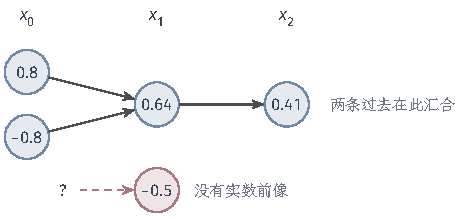
\includegraphics[width=86mm]{figures/03-optimization-evolution-and-signals/02-processes-and-trajectory-evolution/tikz/dds-noninvertible-merge/figure.pdf}
  \caption{不可逆更新$F(x)=x^2$使不同的过去汇合。$x_0=0.8$与$x_0=-0.8$在第一步都到达$0.64$，此后轨道完全相同（$0.64^2\approx0.41$）。负数$-0.5$没有实数前像，因此不能出现在任何轨道的第一步之后。}
  \label{fig:dds-noninvertible-merge}
\end{figure}

这说明离散动力系统的时间方向通常不对称：未来由现在唯一决定，过去却不一定。后面研究长期行为时只使用正向迭代；凡需要往回追溯的地方，例如不变集要求每点都有前像，都会单独说明。

\subsection{历史累计与状态扩充}
\label{sec:dds-history-augmentation}

前两小节从“已有的更新规则需要什么状态”出发。这一小节反过来：先确定希望保留历史的哪些方面，再问能否构造一个有限维状态，让它带着这些信息逐步更新。

\paragraph{有限窗口的累计}
设输入$u_n$是每分钟的加热量，我们想随时知道最近三分钟的总加热量$s_n=u_n+u_{n-1}+u_{n-2}$。能否只用$s_{n-1}$和新输入$u_n$更新$s_n$？写出差就知道不行：
\[
  s_n=s_{n-1}+u_n-u_{n-3},
\]
右边需要即将移出窗口的$u_{n-3}$，它不在$s_{n-1}$中。总和这一个数丢掉了窗口内部的排列，而移出窗口时恰好需要知道最旧的那一项。

闭合的办法是保存整个窗口。令$\bm w_n=(u_n,u_{n-1},u_{n-2})^{\top}$，则
\[
  \bm w_{n+1}=\begin{bmatrix}0&0&0\\1&0&0\\0&1&0\end{bmatrix}\bm w_n+\begin{bmatrix}1\\0\\0\end{bmatrix}u_{n+1},
  \qquad s_n=(1,1,1)\,\bm w_n.
\]
这又是一个线性系统，和图~\ref{fig:dds-state-augmentation}的移位结构相同。代价是维数等于窗口长度$k$：存储和每步计算都随$k$线性增长，窗口取一小时、每秒一个读数时，状态就有$3600$个坐标。

\paragraph{有限统计量未必恢复历史}
若不在乎精确的窗口，而只要一个随时间淡化的平均，就可以用一个数完成闭合更新。\term{指数移动平均}（exponential moving average，EMA）取
\begin{equation}
  m_n=(1-\alpha)\,m_{n-1}+\alpha\,u_n,\qquad 0<\alpha\leq1,
  \label{eq:dds-ema}
\end{equation}
状态只有$m_n$一个坐标，却综合了全部历史：第~\ref{sec:dds-constant-coefficient}小节会把它展开成按$(1-\alpha)^k$衰减的加权和。

一个统计量能闭合地更新，并不意味着它保存了全部有用的历史。

\begin{example}[相同的平均、不同的历史]
\label{ex:dds-ema-insufficient}
取$\alpha=0.5$、$m_0=0$。历史$(u_1,u_2)=(2,0)$给出$m_1=1$、$m_2=0.5$；历史$(0,1)$给出$m_1=0$、$m_2=0.5$。两段历史的EMA相同，此后输入相同则EMA永远相同；但“最近两分钟的总加热量”分别是$2$和$1$，无法从$m_2$读出。
\end{example}

所以状态是否“足够”，取决于我们要预测的是哪一个未来量：$m_n$对它自己的未来是充分的，对窗口总和却不充分。

\paragraph{加权历史的有限基表示}
能不能既只用少数几个坐标，又保留比平均值更丰富的历史形状？一种思路是把整段历史看成一个函数，用少数几个基函数去逼近它，再把展开系数当作状态。离散时间里有一个可以完全算清楚的例子。固定$0<a<1$，定义按距今步数加权的两个矩
\[
  S_0(n)=\sum_{j\leq n}a^{\,n-j}u_j,\qquad
  S_1(n)=\sum_{j\leq n}a^{\,n-j}(n-j)\,u_j,
\]
其中$j$取遍已经发生的时刻。$S_0$是指数加权的总量，$S_1$还按“过去了多久”再加权一次，于是能区分输入集中在近期还是远期。

这两个矩可以闭合地更新。$S_0$的递推$S_0(n)=aS_0(n-1)+u_n$与EMA同型。对$S_1$，把$j=n$的项（权重为$0$）去掉，再把$n-j$写成$(n-1-j)+1$：
\[
  S_1(n)=\sum_{j\leq n-1}a\cdot a^{\,n-1-j}\bigl((n-1-j)+1\bigr)u_j
  =a\bigl(S_1(n-1)+S_0(n-1)\bigr).
\]
合起来，$\bm S(n)=(S_0(n),S_1(n))^{\top}$满足线性递推
\begin{equation}
  \bm S(n)=a\begin{bmatrix}1&0\\1&1\end{bmatrix}\bm S(n-1)+\begin{bmatrix}1\\0\end{bmatrix}u_n .
  \label{eq:dds-moment-state}
\end{equation}
两个坐标足以支撑一个有用的读出：在权重$a^{\,n-j}$下用直线$c_0+c_1(j-n)$拟合历史输入，加权最小二乘的正规方程只涉及两类量：权重的和$\sum_k a^k$、$\sum_k ka^k$、$\sum_k k^2a^k$（只依赖$a$与已经过去的步数，与输入无关），以及数据矩$S_0(n)$、$S_1(n)$。所以拟合直线的截距和斜率都是状态的函数。图~\ref{fig:dds-history-moments}画出一段带噪输入、所用的指数权重，以及仅凭$\bm S(n)$读出的局部直线。

\begin{figure}[htbp]
  \centering
  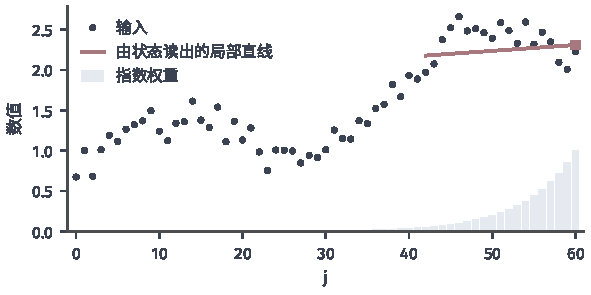
\includegraphics[width=100mm]{figures/03-optimization-evolution-and-signals/02-processes-and-trajectory-evolution/matplotlib/dds-history-moments/figure.pdf}
  \caption{用两个指数加权矩概括历史。黑点为教学用输入$u_j=0.6+0.03j+0.5\sin(j/6)+$噪声（固定随机种子），浅蓝柱为$n=60$时的权重$a^{\,n-j}$，$a=0.85$。红线是只用状态$\bm S(60)=(S_0,S_1)$算出的加权最小二乘直线，方块为其在当前时刻的值。权重集中在最近约十几步，远处的起伏几乎不影响状态。}
  \label{fig:dds-history-moments}
\end{figure}

与均匀窗口对照，可以看出闭合的来源。均匀窗口在左端硬性截断，移出窗口的旧输入必须单独记住；指数权重每步整体乘以$a$，旧输入的影响自动变小，不需要知道它具体是哪一项。所以有限个特征能否自行演化，取决于权重与基的配合，而不是特征个数。

高阶多项式投影（high-order polynomial projection operators，HiPPO）框架系统地发展了这一思路：在连续时间里，选定一个历史测度和一组正交多项式，把到当前为止的输入投影到前$d$个多项式上，并推导投影系数满足的线性方程\scite{gu2020hippo}。不同的测度对应不同的遗忘方式，例如固定长度的滑动窗口或随时间拉长的均匀窗口。连续形式及其离散化留到第~\ref{chap:ordinary-differential-equations}章结合线性状态方程讨论。这里需要分清两项检查：投影误差回答“状态能多准确地重建历史”，状态充分性回答“状态能否决定我们关心的未来”。前者小不保证后者成立，前面EMA的例子已经说明，一个对自身未来充分的状态，仍可能丢掉另一项未来量所需的历史。

% 第1章第2节：线性递推的求解（常系数递推与矩阵幂；时变递推与状态转移）。

\section{线性递推的求解}
\label{sec:dds-linear-recurrences}

一般的非线性递推只能逐步计算。线性和仿射更新则不同：叠加原理让我们把轨迹拆成“初态单独传播”与“每次输入单独传播”两部分，各自写成显式公式。本节先处理系数不随时间变化的情形，这时初态的作用由矩阵幂决定，矩阵的特征值告诉我们各个方向是增长、衰减还是旋转；再处理时变系数，这时必须保留矩阵乘积的先后次序。

\subsection{常系数递推与矩阵幂}
\label{sec:dds-constant-coefficient}

\paragraph{从等比数列到矩阵幂}
最简单的线性递推是标量的$x_{n+1}=ax_n$，它的解是等比数列$x_n=a^nx_0$。$|a|<1$时状态几何衰减，$|a|>1$时几何增长，$a<0$时每步变号，形成来回摆动。温度偏差$x_n-2=0.8^n(x_0-2)$正是$a=0.8$的情形。

向量情形$\bm x_{n+1}=\bm A\bm x_n$的解同样直接：$\bm x_n=\bm A^n\bm x_0$。困难在于读懂$\bm A^n$。矩阵幂的元素一般不是原矩阵元素的幂，例如$\bigl[\begin{smallmatrix}1&1\\0&1\end{smallmatrix}\bigr]^n=\bigl[\begin{smallmatrix}1&n\\0&1\end{smallmatrix}\bigr]$，右上角线性增长，而原矩阵的元素都只有$0$和$1$。要理解长期行为，需要找到让$\bm A$作用变简单的方向。

\paragraph{特征方向：增长、衰减与旋转}
若$\bm A\bm v=\lambda\bm v$，从$\bm v$出发的轨道就是$\lambda^n\bm v$：在特征方向上，矩阵递推退化为标量的等比数列。当$\bm A\in\mathbb R^{d\times d}$有$d$个线性无关的特征向量$\bm v_1,\ldots,\bm v_d$时，把初值分解为$\bm x_0=\sum_ic_i\bm v_i$，得到
\begin{equation}
  \bm x_n=\sum_{i=1}^dc_i\lambda_i^n\bm v_i .
  \label{eq:dds-modal-solution}
\end{equation}
每个分量各自按自己的倍数伸缩，互不干扰。长期看，模最大的特征值主导，只要初值在它的方向上有分量。

想象把所有长度为$1$的初值画成单位圆，再看$\bm A^n$把这个圆变成什么。图~\ref{fig:dds-matrix-power-shapes}(a)中，$\bm A$在水平方向有特征值$1.25$，在对角方向有特征值$0.6$。单位圆被反复作用后，沿水平方向越拉越长，沿对角方向越压越扁，变成一个越来越细长、并逐渐倒向水平特征方向的椭圆。长期看，几乎每个初值都会被拉向增长方向，只有恰好落在对角特征方向上的初值才会衰减到零。

\begin{figure*}[htbp]
  \centering
  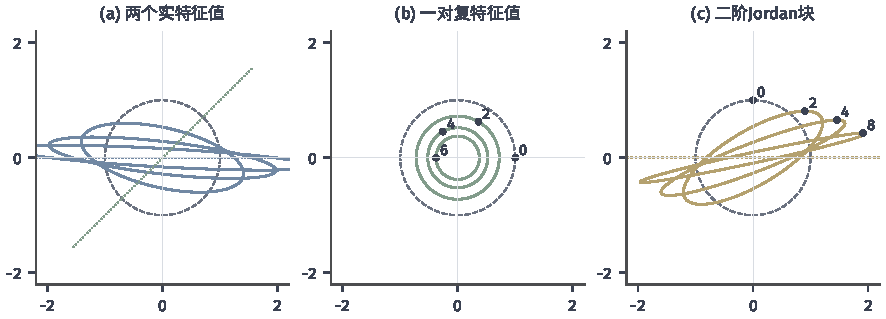
\includegraphics[width=150mm]{figures/03-optimization-evolution-and-signals/02-processes-and-trajectory-evolution/matplotlib/dds-matrix-power-shapes/figure.pdf}
  \caption{矩阵幂对单位圆的作用。虚线为单位圆，实线为它在$\bm A^n$下的像。(a)$\bm A$在水平方向$(1,0)^{\top}$有特征值$1.25$、在对角方向$(1,1)^{\top}$有特征值$0.6$（点线），画$n=1,2,3$：圆被拉长并压扁，倒向增长方向。(b)$\bm A=0.85\,\bm R(\pi/6)$，$\bm R(\varphi)$为逆时针旋转$\varphi$，特征值$0.85\mathrm e^{\pm\mathrm i\pi/6}$，画$n=2,4,6$：圆保持为圆，边旋转边收缩，黑点是$(1,0)^{\top}$的像。(c)$\bm A=\bigl[\begin{smallmatrix}0.9&0.5\\0&0.9\end{smallmatrix}\bigr]$只有一个特征方向（水平点线），画$n=2,4,8$：圆被剪切成斜椭圆，黑点$(0,1)^{\top}$的像先向右远离再缓慢回收。}
  \label{fig:dds-matrix-power-shapes}
\end{figure*}

实矩阵的特征值可以是复数，对应的几何是旋转。设$\lambda=r\mathrm e^{\mathrm i\varphi}$（$r>0$，$0<\varphi<\pi$）是$\bm A$的特征值，复特征向量为$\bm v=\bm p+\mathrm i\bm q$，$\bm p,\bm q\in\mathbb R^d$。比较$\bm A\bm v=\lambda\bm v$两边的实部和虚部，得到
\[
  \bm A\bm p=r(\cos\varphi\,\bm p-\sin\varphi\,\bm q),\qquad
  \bm A\bm q=r(\sin\varphi\,\bm p+\cos\varphi\,\bm q).
\]
因此$\bm p,\bm q$张成的平面在$\bm A$下不变，而在基$(\bm p,\bm q)$下，$\bm A$的作用是把坐标旋转角度$\varphi$（方向由基的取向决定）再乘以$r$。反复作用得到旋转$n\varphi$、缩放$r^n$：轨道沿螺线走向原点（$r<1$）或远离原点（$r>1$）。图~\ref{fig:dds-matrix-power-shapes}(b)是最干净的情形，$\bm A$本身就是$0.85$乘以旋转$\pi/6$。

第~\ref{sec:dds-recurrence-state}小节的动量迭代~\eqref{eq:dds-heavy-ball-state}正是这种情形：它的矩阵没有实特征向量，只有一个旋转缩放的不变平面。

\begin{example}[动量迭代的振荡收敛]
\label{ex:dds-heavy-ball-oscillation}
矩阵$\bigl[\begin{smallmatrix}0.9&-0.4\\1&0\end{smallmatrix}\bigr]$的特征多项式是$\lambda^2-0.9\lambda+0.4$，判别式$0.81-1.6<0$，两根$\lambda=0.45\pm0.4444\mathrm i$。它们的模$r=\sqrt{0.4}\approx0.632$等于两根之积（行列式）的平方根，辐角$\varphi=\arccos(0.45/\sqrt{0.4})\approx44.6^{\circ}$。于是参数$\theta_n$可写成$r^n(C_1\cos n\varphi+C_2\sin n\varphi)$：每步大约转过$45^{\circ}$，约$8$步完成一次振荡，同时振幅每步乘以$0.632$。动量让迭代越过最小点再折回，这在矩阵层面就是一对复特征值。
\end{example}

\paragraph{不可对角化时的多项式因子}
特征向量不够$d$个时，分解~\eqref{eq:dds-modal-solution}不可用，矩阵幂中会出现多项式因子。二维情形已经包含全部机制。考察
\[
  \bm J=\begin{bmatrix}\lambda&1\\0&\lambda\end{bmatrix},\qquad
  \bm J^n=\begin{bmatrix}\lambda^n&n\lambda^{n-1}\\0&\lambda^n\end{bmatrix}.
\]
右式用归纳法验证：$\bm J^n\bm J$的右上角是$\lambda^n+n\lambda^{n-1}\cdot\lambda=(n+1)\lambda^n$。$\bm J$只有一个特征值$\lambda$，而$\bm J-\lambda\bm I$的秩为$1$，所以只有一个特征方向$(1,0)^{\top}$。这样的矩阵称为二阶\term{Jordan块}（Jordan block）。第二个坐标的初值会通过右上角的$1$持续“推”第一个坐标，累计出因子$n$。

多项式因子不会改变最终是增长还是衰减，只改变途中的形状。$|\lambda|<1$时，$n|\lambda|^{n-1}\to0$，因为几何衰减终将压过线性增长；但起初$n$的增长可能占上风。图~\ref{fig:dds-matrix-power-shapes}(c)中$\lambda=0.9$，点$(0,1)^{\top}$的像依次是$(0.5n\cdot0.9^{n-1},\,0.9^n)$：$n=2,4,8$时横坐标约为$0.90$、$1.46$、$1.91$，先远离原点，很久以后才回收。$|\lambda|=1$时多项式因子决定一切：$\lambda=1$给出$\bm J^n=\bigl[\begin{smallmatrix}1&n\\0&1\end{smallmatrix}\bigr]$，特征值的模不超过$1$，矩阵幂却无界。

调整动量迭代的参数，可以让一对复特征值合并成二重实根，恰好落到这种不可对角化的情形。

\begin{example}[临界阻尼的动量迭代]
\label{ex:dds-critical-damping}
把参数改为$\eta=\beta=0.25$，递推成为$\theta_{n+1}=\theta_n-0.25\,\theta_{n-1}$，特征多项式$\lambda^2-\lambda+0.25=(\lambda-0.5)^2$有二重根$0.5$，而相应矩阵$\bigl[\begin{smallmatrix}1&-0.25\\1&0\end{smallmatrix}\bigr]$减去$0.5\bm I$后秩为$1$，只有一个特征方向。直接代入可验证$\theta_n=(c_1+c_2n)\,0.5^n$满足递推：对$\theta_n=n\,0.5^n$，
\[
  \begin{aligned}
  &(n+1)0.5^{n+1}-n\,0.5^n+0.25(n-1)0.5^{n-1}\\
  &\quad=0.5^n\bigl[0.5(n+1)-n+0.5(n-1)\bigr]=0 .
  \end{aligned}
\]
这是“临界阻尼”：复根刚好合并成实二重根，振荡消失，留下一个多项式因子。
\end{example}

一般矩阵可以相似变换成若干Jordan块组成的分块对角形，所以$\bm A^n$的元素总是形如$n^k\lambda^n$的项的线性组合，其中$k$小于相应块的阶数。本章不需要这一完整理论，只用下面的估计。卷一已经证明：对任意$r>\rho(\bm A)$，其中$\rho(\bm A)=\max\{|\lambda|:\lambda\text{为}\bm A\text{的特征值}\}$是\term{谱半径}（spectral radius），存在常数$C_r\geq1$，使
\begin{equation}
  \lVert\bm A^n\rVert\leq C_r\,r^n,\qquad n\geq0,
  \label{eq:dds-geometric-bound}
\end{equation}
等价地，存在$\mathbb R^d$上的一个向量范数，使$\bm A$在它诱导的矩阵范数下不超过$r$。卷一还证明了$\bm A^n\to\bm 0$当且仅当$\rho(\bm A)<1$，以及$\rho(\bm A)=\lim_{n\to\infty}\lVert\bm A^n\rVert^{1/n}$（Gelfand公式）。证明用实Schur形把矩阵化成准上三角形，再用对角缩放把非对角块压小；常数$C_r$正是吸收多项式因子与非正交特征方向的代价，$r$越接近$\rho(\bm A)$，$C_r$可能越大。这些结论与证明可参考\BookChapterRef{chap:linear-analysis}{卷一“谱和奇异值”章}。

\paragraph{输入的累计：注入时刻与剩余传播}
现在加上输入。对常系数系统$\bm x_{n+1}=\bm A\bm x_n+\bm B\bm u_n$，前两步是
\[
  \bm x_1=\bm A\bm x_0+\bm B\bm u_0,\qquad
  \bm x_2=\bm A^2\bm x_0+\bm A\bm B\bm u_0+\bm B\bm u_1 .
\]
规律已经显现：较早的输入被多乘了几次$\bm A$。

\begin{theorem}[常系数仿射递推的显式解]
\label{thm:dds-variation-constants}
设$\bm A\in\mathbb R^{d\times d}$、$\bm B\in\mathbb R^{d\times m}$，$\bm x_0\in\mathbb R^d$，$(\bm u_n)\subseteq\mathbb R^m$。递推$\bm x_{n+1}=\bm A\bm x_n+\bm B\bm u_n$的解为
\begin{equation}
  \bm x_n=\bm A^n\bm x_0+\sum_{j=0}^{n-1}\bm A^{\,n-1-j}\bm B\bm u_j,\qquad n\geq0,
  \label{eq:dds-variation-constants}
\end{equation}
其中$n=0$时求和为空，取零向量。
\end{theorem}

\begin{proof}
$n=0$时右边为$\bm x_0$。设式~\eqref{eq:dds-variation-constants}对某个$n$成立，则
\[
  \begin{aligned}
  \bm x_{n+1}=\bm A\bm x_n+\bm B\bm u_n
  &=\bm A^{n+1}\bm x_0+\sum_{j=0}^{n-1}\bm A^{\,n-j}\bm B\bm u_j+\bm A^0\bm B\bm u_n\\
  &=\bm A^{n+1}\bm x_0+\sum_{j=0}^{n}\bm A^{\,(n+1)-1-j}\bm B\bm u_j .
  \end{aligned}
\]
这正是$n+1$时的公式。
\end{proof}

公式的每一项都有一个“注入—传播”的读法。输入$\bm u_j$在第$j$步注入状态，变成$\bm B\bm u_j$；此后到时刻$n$还要经历$n-1-j$次更新，每次乘以$\bm A$。所以$\bm A^{\,n-1-j}\bm B\bm u_j$是“$j$时刻注入、传播$n-1-j$步”后的残余，状态$\bm x_n$是全部残余与初态残余$\bm A^n\bm x_0$的叠加。图~\ref{fig:dds-input-injection}把标量情形$a=0.8$画成堆叠的面积：每次加热都激起一条按$0.8^k$衰减的“余波”，各条余波叠起来恰好是递推算出的温差。

\begin{figure}[htbp]
  \centering
  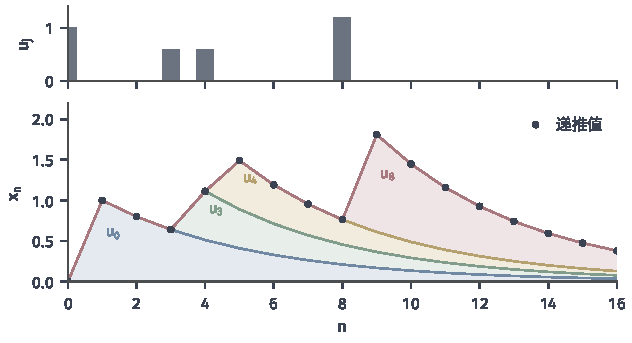
\includegraphics[width=107mm]{figures/03-optimization-evolution-and-signals/02-processes-and-trajectory-evolution/matplotlib/dds-input-injection/figure.pdf}
  \caption{输入的注入与剩余传播。上图为输入序列：$u_0=1$，$u_3=u_4=0.6$，$u_8=1.2$，其余为$0$。下图对$x_{n+1}=0.8x_n+u_n$、$x_0=0$，把每个非零输入的贡献$0.8^{\,n-1-j}u_j$按颜色堆叠；第$j$个输入从$n=j+1$开始出现，此后每步乘以$0.8$。黑点是直接递推得到的$x_n$，与各层之和逐点相同。}
  \label{fig:dds-input-injection}
\end{figure}

公式中“较早的输入被多乘几次$\bm A$”的读法，可以用一个三步的小例子直接核对。

\begin{example}[注入—传播的数值核对]
\label{ex:dds-injection-check}
取$a=1/2$、$b=1$、$x_0=0$，输入$u_0=1$、$u_1=2$、$u_2=1$。逐步递推得$x_1=1$、$x_2=5/2$、$x_3=9/4$。按公式，$x_3=a^2u_0+a\,u_1+u_2=\frac14+1+1=\frac94$：最早的输入传播了两步，只剩四分之一。
\end{example}

零初态时，式~\eqref{eq:dds-variation-constants}是输入序列与固定序列$\bm H_k=\bm A^k\bm B$的离散\term{卷积}（convolution）：$\bm x_n=\sum_{j=0}^{n-1}\bm H_{n-1-j}\bm u_j$。$\bm H_k$描述“单位输入在$k$步以前注入、如今还剩多少”，称为从输入到状态的\term{脉冲响应}（impulse response）。若再读出$\bm y_n=\bm C\bm x_n$，输入到输出的脉冲响应就是$\bm C\bm A^k\bm B$。从卷积和频率的角度研究这种输入—输出关系，是第~\ref{chap:signal-analysis}章的任务；这里只需注意，非零初态的自由响应$\bm A^n\bm x_0$不在卷积之内，必须另外加上。

\paragraph{恒定输入与平衡偏移}
输入恒定为$\bm u$时，若$1$不是$\bm A$的特征值，则$\bm I-\bm A$可逆，方程$\bm x_*=\bm A\bm x_*+\bm B\bm u$有唯一解
\begin{equation}
  \bm x_*=(\bm I-\bm A)^{-1}\bm B\bm u .
  \label{eq:dds-forced-equilibrium}
\end{equation}
用它平移坐标，$\bm x_{n+1}-\bm x_*=\bm A\bm x_n+\bm B\bm u-(\bm A\bm x_*+\bm B\bm u)=\bm A(\bm x_n-\bm x_*)$，所以
\[
  \bm x_n=\bm x_*+\bm A^n(\bm x_0-\bm x_*).
\]
温度例中$x_*=0.4/(1-0.8)=2$，与第~\ref{sec:dds-recurrence-state}小节的计算一致。当$\rho(\bm A)<1$时$\bm A^n\to\bm0$，初态的影响消失，轨迹趋于$\bm x_*$；但$\bm x_*$一般不是零。“初态衰减”与“状态趋零”是两回事：前者只说明系统忘记了从哪里出发，持续施加的输入仍然把状态维持在偏离原点的位置。若$1$是$\bm A$的特征值，平衡可能不存在：标量$a=1$时$x_n=x_0+nu$，任何非零恒定输入都使状态线性增长。

指数移动平均是这一结构的常用实例。递推~\eqref{eq:dds-ema}中令$a=1-\alpha$，由式~\eqref{eq:dds-variation-constants}（时刻从$1$开始计）得
\begin{equation}
  m_n=a^nm_0+\alpha\sum_{j=1}^na^{\,n-j}u_j .
  \label{eq:dds-ema-expansion}
\end{equation}
初值与各次输入的权重之和为$a^n+\alpha(1-a^n)/(1-a)=1$，所以$m_n$是一个加权平均。$k$步以前的输入权重是$\alpha a^k$，降到当前输入权重的$\mathrm e^{-1}$所需的步数为$-1/\ln(1-\alpha)$，$\alpha$较小时约为$1/\alpha$：$\alpha=0.1$时约$9.5$步，$\alpha=0.2$时约$4.5$步。若$m_0=0$只表示“尚无数据”，有限步内观测项的权重之和只有$1-a^n$，把$m_n$除以$1-a^n$可以重新归一化；若$m_0$本身是有效的初始估计，这样做会改变原定的更新。

恒定输入下的平衡还能说明EMA跟踪变化量时的滞后。设输入是匀速上升的$u_j=\mu_0+jd$，记偏差$b_n=m_n-u_n$。由$m_n=am_{n-1}+\alpha u_n$与$u_n=u_{n-1}+d$，
\[
  b_n=a\,m_{n-1}+\alpha u_n-u_n=a\,(m_{n-1}-u_{n-1})-a\,d=a\,b_{n-1}-a\,d .
\]
这是一个系数为$a$、恒定输入为$-ad$的标量递推，平衡为$b_*=-ad/(1-a)=-ad/\alpha$。$\alpha=0.2$时，平均值长期落后真实值$4d$。$\alpha$越小，记忆越长、平滑越强，滞后也越大；平滑与跟踪之间的取舍，在这里成了同一个递推的平衡位置。

\subsection{时变递推与状态转移}
\label{sec:dds-time-varying}

\paragraph{按时间排序的状态转移矩阵}
系数随时间改变时，$\bm x_{n+1}=\bm A_n\bm x_n+\bm B_n\bm u_n$的齐次部分不再是同一个矩阵的幂，而是一串不同矩阵的乘积。为记录“从时刻$m$到时刻$n$”的传播，定义
\begin{equation}
  \bm\Phi(n,m)=\bm A_{n-1}\bm A_{n-2}\cdots\bm A_m\quad(n>m),\qquad
  \bm\Phi(m,m)=\bm I ,
  \label{eq:dds-transition-matrix}
\end{equation}
称为\term{状态转移矩阵}（state transition matrix）。约定$\bm\Phi(m,m)=\bm I$是空乘积的自然取值：不经历任何更新，状态不变。较晚的矩阵写在左边，与复合映射的顺序一致。

由定义直接得到三条性质：$\bm\Phi(n+1,m)=\bm A_n\bm\Phi(n,m)$；对$m\leq k\leq n$有$\bm\Phi(n,m)=\bm\Phi(n,k)\bm\Phi(k,m)$，即先从$m$传播到$k$、再从$k$传播到$n$；齐次轨道满足$\bm x_n=\bm\Phi(n,m)\bm x_m$。与定理~\ref{thm:dds-variation-constants}完全相同的归纳给出非齐次解
\begin{equation}
  \bm x_n=\bm\Phi(n,0)\bm x_0+\sum_{j=0}^{n-1}\bm\Phi(n,j+1)\bm B_j\bm u_j .
  \label{eq:dds-time-varying-solution}
\end{equation}
读法不变：$\bm u_j$在第$j$步注入，此后经历$\bm A_{j+1},\ldots,\bm A_{n-1}$的传播。不同的是，传播核$\bm\Phi(n,j+1)\bm B_j$依赖两个绝对时刻，而不只依赖相隔的步数$n-1-j$；线性还在，平移不变性没有了。

时变系数并不罕见。与第~\ref{sec:dds-history-augmentation}小节的窗口总和不同，从头开始的算术平均可以闭合地更新；它恰好是一个系数随时间变化的线性系统，状态转移矩阵可以直接算出来。

\begin{example}[累计平均作为时变线性系统]
\label{ex:dds-running-mean}
设$m_n=\frac1n\sum_{j=1}^nu_j$是前$n$个输入的平均（$n\geq1$）。由$(n+1)m_{n+1}=nm_n+u_{n+1}$，
\[
  m_{n+1}=\frac{n}{n+1}\,m_n+\frac1{n+1}\,u_{n+1},
\]
系数$a_n=n/(n+1)$随时间变化。从时刻$j$到时刻$n$的转移因子是一串相消的乘积：
\[
  \Phi(n,j)=\frac{n-1}{n}\cdot\frac{n-2}{n-1}\cdots\frac{j}{j+1}=\frac jn .
\]
代入式~\eqref{eq:dds-time-varying-solution}的标量形式（输入$u_{j+1}/(j+1)$在第$j$步注入，传播因子为$\Phi(n,j+1)=(j+1)/n$），每个输入对$m_n$的贡献都是$\frac{j+1}{n}\cdot\frac{u_{j+1}}{j+1}=\frac{u_{j+1}}n$，正是等权平均。与指数移动平均对照：EMA的转移因子$(1-\alpha)^{n-j}$只依赖间隔，旧输入按几何速度被遗忘；累计平均的转移因子$j/n$依赖两个绝对时刻，旧输入的权重随样本增多而按$1/n$均匀稀释，不会被“遗忘”。
\end{example}

乘积的次序不能随意调换，因为一般矩阵不交换。取
\[
  \bm A_0=\begin{bmatrix}1&1\\0&1\end{bmatrix},\quad
  \bm A_1=\begin{bmatrix}1&0\\1&1\end{bmatrix},\qquad
  \bm A_1\bm A_0=\begin{bmatrix}1&1\\1&2\end{bmatrix}\neq
  \begin{bmatrix}2&1\\1&1\end{bmatrix}=\bm A_0\bm A_1 .
\]
次序错了，得到的就是另一个系统的轨迹。

时变还带来一个常见误判：每个时刻的矩阵谱半径都小，不能推出乘积衰减。取交替出现的
\[
  \bm A_{2k}=\begin{bmatrix}0&2\\0&0\end{bmatrix},\qquad
  \bm A_{2k+1}=\begin{bmatrix}0&0\\2&0\end{bmatrix}.
\]
两个矩阵都是幂零的，特征值只有$0$，单独反复使用任何一个，两步之后状态就是零。可是交替使用时，$\bm A_1\bm A_0=\operatorname{diag}(0,4)$，从$\bm x_0=(0,1)^{\top}$出发的轨道是$(2,0)^{\top},(0,4)^{\top},(8,0)^{\top},\ldots$，每步长度翻倍。冻结每个时刻看谱，丢掉了不同时刻的矩阵之间“交接”的方式；时变系统的稳定性必须看整段乘积$\bm\Phi(n,m)$。

\paragraph{仿射更新的结合与并行扫描}
逐步递推是一条严格的串行链：算$\bm x_3$必须先有$\bm x_2$。对长度为$T$的序列，即使有很多处理器，也要依次做$T$步。仿射更新给了一个绕开串行链的机会，关键在于把“一步更新”本身当作可以合并的对象。

把仿射递推$\bm x_{n+1}=\bm A_n\bm x_n+\bm b_n$（$\bm b_n=\bm B_n\bm u_n$已经由给定输入算出）的第$n$步记为二元组$g_n=(\bm A_n,\bm b_n)$，表示映射$\bm x\mapsto\bm A_n\bm x+\bm b_n$。两步复合仍是仿射映射：
\begin{equation}
  (\bm A_2,\bm b_2)\circ(\bm A_1,\bm b_1)=(\bm A_2\bm A_1,\ \bm A_2\bm b_1+\bm b_2).
  \label{eq:dds-affine-composition}
\end{equation}
复合的结果仍是同样大小的二元组，所以任意一段连续更新都能压缩成一个二元组。映射复合满足结合律，三步可以直接核对：
\[
  g_3\circ(g_2\circ g_1)=(\bm A_3\bm A_2\bm A_1,\ \bm A_3\bm A_2\bm b_1+\bm A_3\bm b_2+\bm b_3)=(g_3\circ g_2)\circ g_1 .
\]

结合律允许我们任意安排括号，于是可以用\term{关联扫描}（associative scan，也称前缀扫描）同时求出全部前缀$g_{n-1}\circ\cdots\circ g_0$。把各步更新按时间顺序放在一棵平衡二叉树的叶子上（图~\ref{fig:dds-parallel-scan}）。上行阶段把相邻块两两合并，每个内部节点保存自己整段的总复合；这一阶段结束时只知道整块的总映射，还不知道块内每个前缀。下行阶段从根出发传递“本区间之前已经完成的累计映射”$p$：根接收恒等映射；左孩子原样接收$p$；若左块的总映射为$L$，右孩子接收$L\circ p$。叶子$i$收到的前缀$p_i$恰好是$g_{i-1}\circ\cdots\circ g_0$，再作用$g_i$并代入$\bm x_0$，就得到$\bm x_{i+1}$。右块总是接在左块之后，所以这套规则不需要交换律。

\begin{figure*}[htbp]
  \centering
  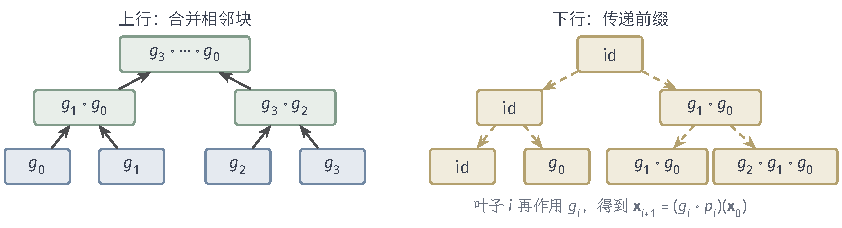
\includegraphics[width=150mm]{figures/03-optimization-evolution-and-signals/02-processes-and-trajectory-evolution/tikz/dds-parallel-scan/figure.pdf}
  \caption{四步仿射更新的关联扫描。左：上行阶段把相邻更新两两复合，每个节点保存所辖区间的总映射，较晚的更新始终写在左边。右：下行阶段从根传入恒等映射，左孩子继承父节点的前缀，右孩子接收“左兄弟的总映射$\circ$父节点前缀”。四个叶子得到的前缀依次是$\mathrm{id}$、$g_0$、$g_1\circ g_0$、$g_2\circ g_1\circ g_0$。同一层的合并互不依赖，可以同时进行。}
  \label{fig:dds-parallel-scan}
\end{figure*}

代价要分开计算。总工作量数所有节点上执行的合并次数，计算深度数最长依赖链上的合并次数。$T$步形成的平衡树有$O(T)$个节点、$O(\log T)$层，上行和下行在每个节点只做常数次合并，同层节点互不依赖。所以把一次合并算作一个操作时，总工作量为$O(T)$，\term{并行深度}（parallel depth）为$O(\log T)$，而顺序递推的深度是$T$。但一次合并的实际算术量取决于矩阵形式：一般稠密的$d\times d$矩阵相乘需要$O(d^3)$次运算，而顺序递推每步只需$O(d^2)$的矩阵乘向量，所以扫描用更多的总运算换取更短的深度。若$\bm A_n$都是对角矩阵，合并只需$O(d)$次运算，两种做法的总量同阶。线性状态空间序列模型常把转移矩阵取成对角形式并用这种扫描训练，原因即在于此\scite{gu2023mamba}。扫描还要保存树上的中间二元组，存储量为$O(T)$个二元组。

两点限制需要记住。第一，结合律保证的是精确算术下的结果相同，浮点运算改变括号会改变舍入：双精度下$(1+10^{17})-10^{17}=0$，而$1+(10^{17}-10^{17})=1$。长乘积或条件数较大的传播尤其敏感，所以并行实现应按误差容限验证，不能要求与顺序递推逐位相同。第二，扫描要求每一步的$(\bm A_n,\bm b_n)$事先已知。若系数依赖尚未算出的状态，例如$\bm A_n=\bm A(\bm x_n)$，就不能预先组成二元组；若复合后不再有固定大小的表示，压缩整段更新的前提也就不存在。

% 第1章第3节：平衡、周期与稳定性（平衡点与周期轨道；线性稳定与局部线性化；Lyapunov函数与吸引区域）。

\section{平衡、周期与稳定性}
\label{sec:dds-equilibria-stability}
\label{sec:dynamical-stability-sensitivity}

真实系统很少恰好从理想状态出发：初值有测量误差，运行中也会受到扰动。所以除了“轨迹去往哪里”，更要紧的是“出发点稍有偏差时，轨迹还去不去那里”。本节先找出不随时间改变的状态和周而复始的状态，再把“偏差不放大”“偏差最终消失”“偏差按几何速率消失”写成三种稳定性，最后按系统的结构给出判据：线性系统看谱半径，非线性系统先在平衡点处线性化，线性化不能回答时再寻找每步下降的Lyapunov函数。

\subsection{平衡点与周期轨道}
\label{sec:dds-equilibria-periodic}

\paragraph{平衡点}
温度模型在$x_*=2$处停住，是因为把$2$代入更新规则仍得到$2$。一般地，自治系统$x_{n+1}=F(x_n)$中满足
\begin{equation}
  F(x_*)=x_*
  \label{eq:dds-fixed-point}
\end{equation}
的状态称为\term{平衡点}（equilibrium point），也就是映射$F$的\term{不动点}（fixed point）。从平衡点出发的轨道永远停在那里。恒定输入的系统先把输入代入$F$，再按式~\eqref{eq:dds-fixed-point}求解，例如式~\eqref{eq:dds-forced-equilibrium}。

求平衡点是代数问题。Logistic映射~\eqref{eq:dds-logistic}的方程$x=rx(1-x)$化为$x\bigl(rx-(r-1)\bigr)=0$，解为$x=0$和$x_r=1-1/r$；后者在$r\geq1$时才落在$[0,1]$中。但求出平衡点只说明“停在那里就不会动”，没有说明附近的轨道会不会靠过来。$F(x)=2x$以$0$为平衡点，任何非零初值却都以倍增的速度离开它。平衡点的存在与它的稳定性必须分开讨论。

\paragraph{周期点与最小周期}
轨道还可能不停下来，而是周而复始。若$F^p(x)=x$（$p\geq1$），称$x$为周期$p$的点；使之成立的最小正整数$p$称为$x$的最小周期。此时轨道$x,F(x),\ldots,F^{p-1}(x)$两两不同，并按这个顺序循环，这$p$个点组成一条\term{周期轨道}（periodic orbit）。平衡点就是最小周期为$1$的点。

“最小”二字需要单独检查，因为平衡点满足$F^p(x_*)=x_*$对一切$p$成立。以Logistic映射的周期二为例，$F_r^2(x)=x$是关于$x$的四次方程，它的根包含两个平衡点$0$和$x_r$。把这两个因子除去，剩下二次方程
\[
  r^2x^2-r(r+1)x+(r+1)=0,\qquad
  x_\pm=\frac{(r+1)\pm\sqrt{(r+1)(r-3)}}{2r}.
\]
它在$r>3$时有两个不同的实根，且两根都不是平衡点，于是$\{x_-,x_+\}$是一条最小周期为二的轨道；$r=3$时两根重合为$x_r=2/3$，不再给出新的周期轨道。取$r=3.2$，算得$x_-\approx0.5130$、$x_+\approx0.7995$，代入可验证$F_{3.2}(x_-)=x_+$、$F_{3.2}(x_+)=x_-$。图~\ref{fig:dds-period-two-graph}把$F$与$F^2$画在一起：$F^2$与对角线有四个交点，其中两个是$F$的平衡点，另外两个就是周期二的点。

\begin{figure}[htbp]
  \centering
  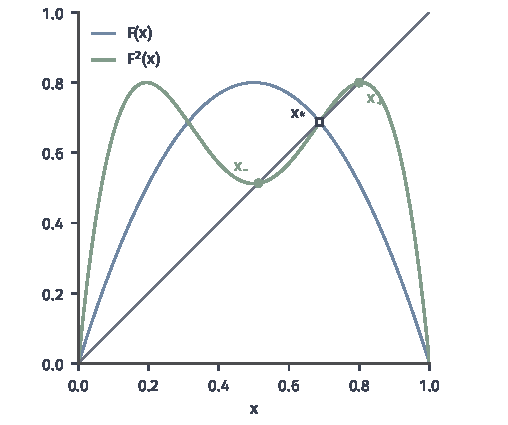
\includegraphics[width=80mm]{figures/03-optimization-evolution-and-signals/02-processes-and-trajectory-evolution/matplotlib/dds-period-two-graph/figure.pdf}
  \caption{$r=3.2$时Logistic映射$F$（蓝）与两步映射$F^2$（绿）。$F^2$与对角线的交点是$F^2$的不动点：$0$与$x_*=0.6875$同时也是$F$的不动点（方块标出$x_*$），$x_-\approx0.513$与$x_+\approx0.799$则组成最小周期为二的轨道。在$x_*$处$F^2$的斜率大于$1$，在$x_\pm$处斜率的绝对值小于$1$。}
  \label{fig:dds-period-two-graph}
\end{figure}

\paragraph{蛛网图：在函数图像上读轨道}
一维映射的轨道可以直接画在$F$的图像上，不必列出数表。在同一坐标系中画$y=F(x)$和对角线$y=x$。从$(x_0,x_0)$出发，竖直走到图像上的$(x_0,F(x_0))=(x_0,x_1)$，再水平走到对角线上的$(x_1,x_1)$，然后重复。竖直一步是“计算下一个值”，水平一步是“把输出当作新的输入”。这样画出的折线称为蛛网图。平衡点正是图像与对角线的交点。

图~\ref{fig:dds-cobweb}用蛛网图比较三种长期行为。(a)中$r=2.8$，折线绕着交点$x_r\approx0.643$一圈圈收紧，轨道收敛到平衡点；之所以是绕圈而不是单侧靠近，是因为该处图像的斜率$F'(x_r)=2-r=-0.8$为负，每一步都跳到平衡点的另一侧。(b)中$r=3.2$，折线不再收向交点，而是收向一个正方形，即周期二轨道$\{x_-,x_+\}$。(c)中$F(x)=x^2$在$x_*=1$处斜率为$2$，从$1.05$出发的轨道远离而去，从$0.95$出发的轨道离开$1$后滑向另一个平衡点$0$。

\begin{figure*}[htbp]
  \centering
  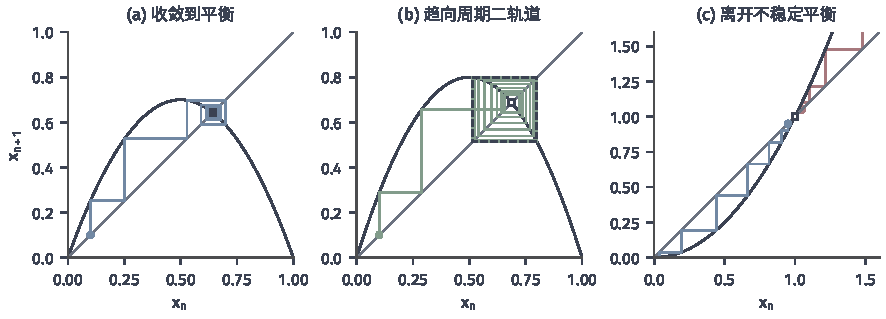
\includegraphics[width=150mm]{figures/03-optimization-evolution-and-signals/02-processes-and-trajectory-evolution/matplotlib/dds-cobweb/figure.pdf}
  \caption{三种长期行为的蛛网图。黑色曲线为$y=F(x)$，灰线为对角线，圆点为初值。(a)Logistic映射$r=2.8$、$x_0=0.1$，轨道绕平衡点$x_r=1-1/r$收紧。(b)$r=3.2$、$x_0=0.1$，轨道趋向虚线方框所示的周期二轨道，空心方块是已经失稳的平衡点$0.6875$。(c)$F(x)=x^2$，空心方块为$x_*=1$；红色从$1.05$出发并无界增长，蓝色从$0.95$出发并趋于$0$。}
  \label{fig:dds-cobweb}
\end{figure*}

\paragraph{周期轨道化为$p$步映射的不动点}
周期轨道的稳定性不需要新的理论。周期$p$的点是$G=F^p$的不动点，所以“附近的轨道是否回到这条周期轨道”可以转化为“$G$的这个不动点是否稳定”，下一小节的判据对$G$照样适用。对可微的一维映射，由链式法则，
\begin{equation}
  (F^p)'(x_0)=F'(x_{p-1})\,F'(x_{p-2})\cdots F'(x_0),
  \label{eq:dds-period-multiplier}
\end{equation}
右边是沿整条周期轨道的导数之积，与从哪一点开始无关。所以同一条周期轨道上的各点要么一起稳定，要么一起不稳定。这个乘积称为周期轨道的乘子，图~\ref{fig:dds-period-two-graph}中$F^2$在$x_\pm$处的斜率就是它。

\subsection{线性稳定与局部线性化}
\label{sec:dds-linear-stability}

\paragraph{三种稳定性}
设$X\subseteq\mathbb R^d$，$F:X\to X$连续，$\bm x_*$是平衡点，$\lVert\cdot\rVert$是$\mathbb R^d$上的一个范数。“偏差不放大”和“偏差最终消失”是两个不同的要求：前者限制整个未来的最大偏差，后者只管最终去向。再加上速度要求，就得到下面三种性质。

\begin{definition}[平衡点的稳定性]
\label{def:dds-stability}
\begin{enumerate}
  \item 若对每个$\varepsilon>0$存在$\delta>0$，使$\lVert\bm x_0-\bm x_*\rVert<\delta$蕴含$\lVert\bm x_n-\bm x_*\rVert<\varepsilon$对全部$n\geq0$成立，称$\bm x_*$在Lyapunov意义下\term{稳定}（stable）。
  \item 若$\bm x_*$稳定，且存在$r>0$，使$\lVert\bm x_0-\bm x_*\rVert<r$蕴含$\bm x_n\to\bm x_*$，称$\bm x_*$\term{渐近稳定}（asymptotically stable）。后一条件单独称为局部吸引。
  \item 若存在$r>0$、$C\geq1$与$0\leq q<1$，使$\lVert\bm x_0-\bm x_*\rVert<r$蕴含
  \[
    \lVert\bm x_n-\bm x_*\rVert\leq C\,q^n\,\lVert\bm x_0-\bm x_*\rVert,\qquad n\geq0,
  \]
  称$\bm x_*$\term{指数稳定}（exponentially stable）。
\end{enumerate}
若吸引条件或指数估计对全部$\bm x_0\in X$成立，相应地称为全局渐近稳定或全局指数稳定。
\end{definition}

量词的位置决定了各项的含义。稳定性是对每个容许偏差$\varepsilon$找初值半径$\delta$，要求整个未来都在$\varepsilon$之内，而不只是最终回来；吸引只要求最终趋于$\bm x_*$，途中可以走得很远；指数稳定要求常数$C,q$对邻域内全部初值统一。有限维空间上范数彼此等价，所以三种性质与所选范数无关，换范数只改变$\delta$和$C$。展示一条收敛的轨迹不能代替这些对整个邻域的陈述。

三个标量例子说明这些性质确实不同，原点都是平衡点。$x_{n+1}=x_n$：每个初值保持不动，原点稳定但不吸引。$x_{n+1}=x_n-x_n^3$：当$0<|x_0|\leq1$时$|x_{n+1}|=|x_n|(1-x_n^2)<|x_n|$，轨道单调地趋于$0$，原点渐近稳定；但衰减很慢，$x_0=0.5$时$x_{100}\approx0.069$、$x_{1000}\approx0.022$，大致与$1/\sqrt{2n}$相符，相邻两步之比$1-x_n^2\to1$，不存在统一的几何速率，所以不是指数稳定。$x_{n+1}=0.5x_n$：$|x_n|=0.5^n|x_0|$，全局指数稳定。

\paragraph{线性定常系统的谱判据}
对线性系统$\bm x_{n+1}=\bm A\bm x_n$，原点总是平衡点，轨道$\bm A^n\bm x_0$又有第~\ref{sec:dds-constant-coefficient}小节的显式描述，所以三种稳定性都能化成矩阵幂的条件。线性还带来一个简化：缩放初值等于缩放整条轨道，局部性质与全局性质没有区别。

\begin{theorem}[离散线性定常系统的稳定性判据]
\label{thm:dynamical-discrete-spectral-stability}
\label{thm:dds-spectral-stability}
设$\bm A\in\mathbb R^{d\times d}$，考察$\bm x_{n+1}=\bm A\bm x_n$的平衡点$\bm 0$。
\begin{enumerate}
  \item $\bm 0$稳定，当且仅当$\sup_{n\geq0}\lVert\bm A^n\rVert<\infty$。
  \item $\bm 0$渐近稳定，当且仅当$\rho(\bm A)<1$。此时$\bm 0$全局指数稳定：对任意$q\in(\rho(\bm A),1)$，存在$C\geq1$，使$\lVert\bm A^n\bm x_0\rVert\leq Cq^n\lVert\bm x_0\rVert$对全部$\bm x_0$与$n\geq0$成立。
\end{enumerate}
\end{theorem}

\begin{proof}
(1) 若$M=\sup_n\lVert\bm A^n\rVert<\infty$，对给定$\varepsilon$取$\delta=\varepsilon/M$，则$\lVert\bm x_0\rVert<\delta$时$\lVert\bm A^n\bm x_0\rVert\leq M\lVert\bm x_0\rVert<\varepsilon$。反之，若$\bm 0$稳定，取$\varepsilon=1$得到相应的$\delta$。对任意单位向量$\bm v$，$\lVert(\delta/2)\bm v\rVert<\delta$，所以$\lVert\bm A^n(\delta/2)\bm v\rVert<1$，即$\lVert\bm A^n\bm v\rVert<2/\delta$。对全部单位向量取上确界，得$\lVert\bm A^n\rVert\leq2/\delta$对全部$n$成立。

(2) 设$\rho(\bm A)<1$，任取$q\in(\rho(\bm A),1)$，由估计~\eqref{eq:dds-geometric-bound}得$\lVert\bm A^n\rVert\leq Cq^n$。这同时给出全局指数稳定、全局吸引，以及(1)中的有界性，从而渐近稳定。反之，设$\bm 0$渐近稳定，相应的吸引半径为$r$。对任意$\bm x_0\neq\bm 0$，$\bm y_0=(r/2)\bm x_0/\lVert\bm x_0\rVert$落在吸引邻域内，所以$\bm A^n\bm y_0\to\bm 0$；由线性，$\bm A^n\bm x_0=(2\lVert\bm x_0\rVert/r)\bm A^n\bm y_0\to\bm 0$。取$\bm x_0$为各个标准基向量，得$\bm A^n$的每一列趋于零，即$\bm A^n\to\bm 0$，再由第~\ref{sec:dds-constant-coefficient}小节所引的判据得$\rho(\bm A)<1$。
\end{proof}

谱半径严格小于$1$的矩阵称为\term{Schur稳定}（Schur stable）矩阵。定理说明，对线性系统，渐近稳定、全局渐近稳定和指数稳定是同一件事；它们都由特征值是否全部严格落在单位圆内决定。

谱半径等于$1$是临界情形，结果取决于单位圆上特征值的结构，不能只看谱半径。旋转矩阵$\bm R(\varphi)$的特征值是$\mathrm e^{\pm\mathrm i\varphi}$，$\lVert\bm R(\varphi)^n\rVert_2=1$，原点稳定但不吸引；$\operatorname{diag}(1,-1)$也稳定，轨道在两点之间来回翻转。而第~\ref{sec:dds-constant-coefficient}小节的$\bm J=\bigl[\begin{smallmatrix}1&1\\0&1\end{smallmatrix}\bigr]$同样只有特征值$1$，$\bm J^n$的右上角却是$n$，由定理的(1)，原点不稳定。一般结论是：$\sup_n\lVert\bm A^n\rVert<\infty$当且仅当$\rho(\bm A)\leq1$，且每个模为$1$的特征值的几何重数等于代数重数，也就是它对应的Jordan块都是一阶的；这可由Jordan标准形逐块计算矩阵幂得到，本章只用上面的二维例子说明机制。

时变系统不能套用这个判据。第~\ref{sec:dds-time-varying}小节交替使用两个幂零矩阵的例子中，每一步的谱半径都是$0$，轨道却每步翻倍。

\paragraph{非线性映射的局部线性化}
非线性映射一般没有显式解，但在平衡点附近，可微映射与它的线性部分相差很小。设$F$在$\bm x_*$的邻域内可微，记\term{Jacobian矩阵}（Jacobian matrix）$\bm J=DF(\bm x_*)$，则
\[
  F(\bm x)-\bm x_*=\bm J(\bm x-\bm x_*)+\bm\rho(\bm x),\qquad
  \frac{\lVert\bm\rho(\bm x)\rVert}{\lVert\bm x-\bm x_*\rVert}\to0\quad(\bm x\to\bm x_*).
\]
偏差$\bm e_n=\bm x_n-\bm x_*$近似满足线性递推$\bm e_{n+1}\approx\bm J\bm e_n$。用$\bm J$判断平衡点的稳定性，就是\term{线性化}（linearization）。可微、Jacobian矩阵与余项的性质可参考\BookChapterRef{chap:multivariate-calculus}{卷一“多元函数微分”章}。下面的定理说明，只要$\bm J$的谱不落在单位圆上，线性化给出的结论就是对的。

\begin{theorem}[线性化判据]
\label{thm:dds-linearization}
设$U\subseteq\mathbb R^d$为开集，$F:U\to\mathbb R^d$在平衡点$\bm x_*\in U$处可微，$\bm J=DF(\bm x_*)$。
\begin{enumerate}
  \item 若$\rho(\bm J)<1$，则$\bm x_*$指数稳定。
  \item 若$\bm J$有模大于$1$的特征值，则$\bm x_*$不稳定。
\end{enumerate}
\end{theorem}

\begin{proof}
(1) 取$\rho(\bm J)<q_1<q<1$。由第~\ref{sec:dds-constant-coefficient}小节所引的范数构造，存在$\mathbb R^d$上的范数$\lVert\cdot\rVert_*$，使$\bm J$在其诱导矩阵范数下满足$\lVert\bm J\rVert_*\leq q_1$。由可微性，存在$r>0$，使$\lVert\bm x-\bm x_*\rVert_*<r$时$\bm x\in U$且$\lVert\bm\rho(\bm x)\rVert_*\leq(q-q_1)\lVert\bm x-\bm x_*\rVert_*$。于是在这个球内
\[
  \lVert F(\bm x)-\bm x_*\rVert_*\leq\lVert\bm J\rVert_*\lVert\bm x-\bm x_*\rVert_*+(q-q_1)\lVert\bm x-\bm x_*\rVert_*\leq q\,\lVert\bm x-\bm x_*\rVert_*.
\]
右边小于$r$，所以$F$把球映回自身；归纳得$\lVert\bm x_n-\bm x_*\rVert_*\leq q^n\lVert\bm x_0-\bm x_*\rVert_*$。由范数等价，存在$c_1,c_2>0$使$c_1\lVert\cdot\rVert\leq\lVert\cdot\rVert_*\leq c_2\lVert\cdot\rVert$，于是对$\lVert\bm x_0-\bm x_*\rVert<r/c_2$有$\lVert\bm x_n-\bm x_*\rVert\leq(c_2/c_1)q^n\lVert\bm x_0-\bm x_*\rVert$，这就是指数稳定。

(2) 不妨设$\bm x_*=\bm 0$。记$\mu_0=\min\{|\lambda|:|\lambda|>1\}$，取$\mu\in(1,\mu_0)$使$\bm J$没有模等于$\mu$的特征值。按特征值的模大于或小于$\mu$，$\mathbb R^d$分解为两个$\bm J$不变子空间的直和$E_u\oplus E_c$，$E_u\neq\{\bm 0\}$；这是线性代数中按特征值分组的不变子空间分解。记$\bm J_u,\bm J_c$为$\bm J$在两个子空间上的限制，则$\bm J_u$可逆，$\rho(\bm J_u^{-1})<1/\mu$，$\rho(\bm J_c)<\mu$。取$1<b<a$使$\rho(\bm J_c)<b<\mu<a$且$\rho(\bm J_u^{-1})<1/a$，再像(1)那样在两个子空间上分别取范数，使$\lVert\bm J_c\bm v\rVert\leq b\lVert\bm v\rVert$、$\lVert\bm J_u\bm w\rVert\geq a\lVert\bm w\rVert$。把$\bm x=\bm w+\bm v$（$\bm w\in E_u$，$\bm v\in E_c$）的范数定义为$\lVert\bm w\rVert+\lVert\bm v\rVert$，并考虑锥形区域$K=\{\lVert\bm v\rVert\leq\lVert\bm w\rVert\}$。

令$\gamma=(a-b)/4$，取$r>0$使$\lVert\bm x\rVert<r$时$\bm x\in U$且余项满足$\lVert\bm\rho(\bm x)\rVert\leq\gamma\lVert\bm x\rVert$；按所取范数的定义，余项在$E_u$、$E_c$上的两个分量的范数都不超过$\lVert\bm\rho(\bm x)\rVert$。对$\bm x\in K$且$\lVert\bm x\rVert<r$，有$\lVert\bm x\rVert\leq2\lVert\bm w\rVert$，于是$F(\bm x)$的两个分量满足
\[
  \lVert\bm w'\rVert\geq a\lVert\bm w\rVert-2\gamma\lVert\bm w\rVert,\qquad
  \lVert\bm v'\rVert\leq b\lVert\bm v\rVert+2\gamma\lVert\bm w\rVert\leq(b+2\gamma)\lVert\bm w\rVert .
\]
因为$a-2\gamma=b+2\gamma=(a+b)/2>1$，所以$F(\bm x)\in K$且$\lVert\bm w'\rVert\geq\kappa\lVert\bm w\rVert$，$\kappa=(a+b)/2>1$。于是从$K$中任意小的非零初值（例如$\bm x_0=\bm w_0\in E_u$）出发，只要轨道还在半径$r$的球内，$E_u$分量就每步至少乘以$\kappa$，因而有限步内必然离开这个球。取$\varepsilon=r$，不存在满足稳定性定义的$\delta$。
\end{proof}

定理把非线性问题的大部分情形交给了线性代数。下面把它用在贯穿本节的Logistic映射上。

\begin{example}[Logistic映射的平衡点与周期二轨道]
\label{ex:dds-logistic-linearization}
$F_r'(x)=r(1-2x)$，在平衡点$x_r=1-1/r$处$F_r'(x_r)=2-r$。所以$1<r<3$时$|2-r|<1$，$x_r$指数稳定；$r>3$时$F_r'(x_r)<-1$，$x_r$不稳定，这正是图~\ref{fig:dds-cobweb}(a)(b)之间发生的变化。对周期二轨道，把定理用于$F_r^2$，由式~\eqref{eq:dds-period-multiplier}与$x_++x_-=(r+1)/r$、$x_+x_-=(r+1)/r^2$，
\[
  (F_r^2)'(x_\pm)=r^2(1-2x_+)(1-2x_-)=r^2-2r(r+1)+4(r+1)=-r^2+2r+4 .
\]
$r=3.2$时乘子为$0.16$，周期二轨道稳定，与蛛网图一致。第~\ref{sec:dds-bifurcation}小节将跟踪这个乘子随$r$的变化。
\end{example}

谱落在单位圆上时，线性化无法下结论，必须看高阶项。$x_{n+1}=x_n-x_n^3$与$x_{n+1}=x_n+x_n^3$在原点的导数都是$1$；前者原点渐近稳定（前面已经算过），后者从任何$x_0>0$出发都单调增长并离开原点，原点不稳定。同样的线性部分，长期行为相反。

\paragraph{长期衰减与瞬态放大}
谱判据描述$n\to\infty$时的行为，对有限步内发生什么说得很少。考察
\[
  \bm A_K=\begin{bmatrix}0.5&K\\0&0.5\end{bmatrix},\qquad
  \bm A_K^n=\begin{bmatrix}0.5^n&2nK\,0.5^{n}\\0&0.5^n\end{bmatrix}.
\]
无论$K$多大，谱半径都是$0.5$，原点全局指数稳定。从$\bm x_0=(0,1)^{\top}$出发，$K=4$时第一步就到达$(4,0.5)^{\top}$，欧氏长度约$4.03$，第二步约$4.01$，第三步约$3.00$，直到第六步才回到初始长度$1$以下（图~\ref{fig:dds-transient-growth}）。放大不来自输入，也不来自数值误差，而来自第二个坐标通过$K$对第一个坐标的持续推动，即前面Jordan块中多项式因子$n$的作用。

\begin{figure}[htbp]
  \centering
  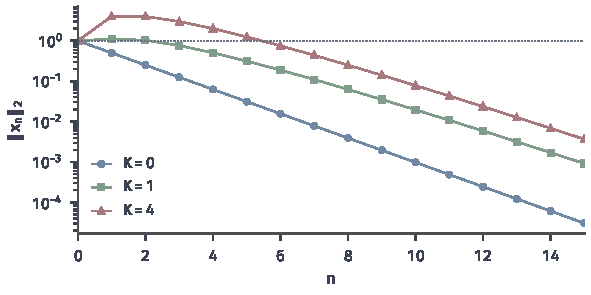
\includegraphics[width=100mm]{figures/03-optimization-evolution-and-signals/02-processes-and-trajectory-evolution/matplotlib/dds-transient-growth/figure.pdf}
  \caption{同一谱半径下的不同瞬态。对$\bm A_K=\bigl[\begin{smallmatrix}0.5&K\\0&0.5\end{smallmatrix}\bigr]$与$\bm x_0=(0,1)^{\top}$，画出$\lVert\bm A_K^n\bm x_0\rVert_2$，纵轴取对数，点线为初始长度$1$。三条曲线的谱半径都是$0.5$，长期斜率相同；$K=1$时第一步长度约$1.12$，$K=4$时前两步约$4.03$与$4.01$。}
  \label{fig:dds-transient-growth}
\end{figure}

$K\neq0$时$\bm A_K\bm A_K^{\top}\neq\bm A_K^{\top}\bm A_K$，矩阵不是\term{正规矩阵}（normal matrix）。正规矩阵可由正交矩阵对角化，满足$\lVert\bm A^n\rVert_2=\rho(\bm A)^n$，不会出现瞬态放大；非正规矩阵的特征方向不正交，甚至不够用，初值可能是几个很长、方向几乎相反的分量相消的结果，分量以不同速度衰减时相消被打破，长度便先增后减。工程上若中间状态不得越过某个边界，例如温度不得超过安全上限，仅凭谱半径小于$1$不能保证安全，还需要直接估计有限步的增益$\lVert\bm A^n\rVert$。

\subsection{Lyapunov函数与吸引区域}
\label{sec:dds-lyapunov}

\paragraph{换一把尺子：二次Lyapunov函数}
图~\ref{fig:dds-transient-growth}提出一个问题：既然欧氏长度不是每步下降，能不能换一种“长度”，使它沿每条轨道都严格下降？如果能，稳定性就可以一步一步地验证，而不必计算整个矩阵幂。对线性系统，自然的候选是二次型$V(\bm x)=\bm x^{\top}\bm P\bm x$，其中$\bm P\succ\bm0$对称正定，它的水平集是一族椭圆。沿$\bm x_{n+1}=\bm A\bm x_n$的一步变化为
\[
  V(\bm A\bm x)-V(\bm x)=\bm x^{\top}(\bm A^{\top}\bm P\bm A-\bm P)\bm x .
\]
要求它对每个非零$\bm x$为负，就是要求$\bm A^{\top}\bm P\bm A-\bm P$负定。

\begin{theorem}[离散Lyapunov方程]
\label{thm:dynamical-discrete-lyapunov-equation}
\label{thm:dds-discrete-lyapunov-equation}
设$\bm A\in\mathbb R^{d\times d}$。以下三条等价：
\begin{enumerate}
  \item $\rho(\bm A)<1$，即$\bm A$是Schur稳定矩阵；
  \item 对每个对称正定矩阵$\bm Q$，方程
  \begin{equation}
    \bm A^{\top}\bm P\bm A-\bm P=-\bm Q
    \label{eq:dds-discrete-lyapunov}
  \end{equation}
  在$\mathbb R^{d\times d}$中有唯一解$\bm P$，且$\bm P$对称正定；
  \item 存在对称正定矩阵$\bm P$与$\bm Q$满足方程~\eqref{eq:dds-discrete-lyapunov}。
\end{enumerate}
\end{theorem}

\begin{proof}
(1)$\Rightarrow$(2)：取$q\in(\rho(\bm A),1)$，由估计~\eqref{eq:dds-geometric-bound}，$\lVert(\bm A^{\top})^k\bm Q\bm A^k\rVert\leq\lVert\bm Q\rVert C^2q^{2k}$（矩阵范数取谱范数，$\lVert\bm A^{\top k}\rVert_2=\lVert\bm A^k\rVert_2$），所以级数
\[
  \bm P=\sum_{k=0}^{\infty}(\bm A^{\top})^k\bm Q\bm A^k
\]
绝对收敛。每一项对称，$\bm P$对称；首项$\bm Q$正定、其余各项半正定，故$\bm P\succeq\bm Q\succ\bm0$。代入验证：$\bm A^{\top}\bm P\bm A=\sum_{k\geq1}(\bm A^{\top})^k\bm Q\bm A^k=\bm P-\bm Q$。若$\bm P'$是另一个解（不必对称），差$\bm D=\bm P-\bm P'$满足$\bm D=\bm A^{\top}\bm D\bm A$，反复代入得$\bm D=(\bm A^{\top})^n\bm D\bm A^n\to\bm0$，故$\bm D=\bm0$。

(2)$\Rightarrow$(3)：取$\bm Q=\bm I$即可。

(3)$\Rightarrow$(1)：设$\lambda\in\mathbb C$是$\bm A$的特征值，$\bm v\in\mathbb C^d$为相应的非零特征向量，$\bm v^*$表示共轭转置。对方程~\eqref{eq:dds-discrete-lyapunov}左乘$\bm v^*$、右乘$\bm v$，由$\bm A\bm v=\lambda\bm v$得
\[
  (|\lambda|^2-1)\,\bm v^*\bm P\bm v=-\bm v^*\bm Q\bm v .
\]
实对称正定矩阵对非零复向量也给出正的二次型：写$\bm v=\bm a+\mathrm i\bm b$，则$\bm v^*\bm P\bm v=\bm a^{\top}\bm P\bm a+\bm b^{\top}\bm P\bm b>0$，对$\bm Q$同理。所以$|\lambda|^2-1<0$。这对每个特征值成立，故$\rho(\bm A)<1$。
\end{proof}

方程~\eqref{eq:dds-discrete-lyapunov}又称Stein方程，它是关于$\bm P$的线性方程组，规模较大时有利用Schur分解的专门解法，可参考\BookChapterRef{chap:linear-equations-and-optimization}{卷一“线性方程与矩阵方程”章}。小规模时可以手算，并且手算能看清每个未知数从哪个方程来。

\begin{example}[二阶Stein方程的手算]
\label{ex:dds-stein-by-hand}
取前面的$\bm A_1=\bigl[\begin{smallmatrix}0.5&1\\0&0.5\end{smallmatrix}\bigr]$、$\bm Q=\bm I$，设$\bm P=\bigl[\begin{smallmatrix}p&s\\s&t\end{smallmatrix}\bigr]$。方程逐元素给出
\[
  0.25p-p=-1,\qquad 0.5p+0.25s-s=0,\qquad p+s+0.25t-t=-1,
\]
依次解得$p=4/3$、$s=8/9$、$t=116/27\approx4.30$。$\bm P$的特征值约为$1.09$和$4.54$，确实正定。
\end{example}

这个$\bm P$给出了一把倾斜的尺子。图~\ref{fig:dds-lyapunov-ellipses}(a)画出$V$的若干水平椭圆和从$(0,1)^{\top}$出发的轨道：第一步到达$(1,0.5)^{\top}$，越出了单位圆，欧氏长度从$1$增至$1.118$；但它落在更内层的椭圆上，$V$从$4.30$降到$3.30$，恰好减少$\bm x_0^{\top}\bm Q\bm x_0=1$。(b)比较两种长度：$\sqrt V$每步下降，欧氏长度则先升后降。

\begin{figure}[htbp]
  \centering
  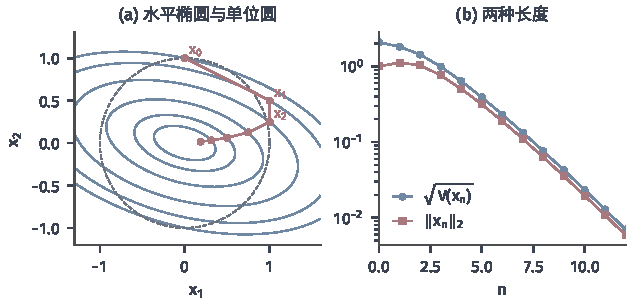
\includegraphics[width=107mm]{figures/03-optimization-evolution-and-signals/02-processes-and-trajectory-evolution/matplotlib/dds-lyapunov-ellipses/figure.pdf}
  \caption{二次Lyapunov函数作为倾斜的尺子。$\bm A=\bigl[\begin{smallmatrix}0.5&1\\0&0.5\end{smallmatrix}\bigr]$，$\bm P$由$\bm A^{\top}\bm P\bm A-\bm P=-\bm I$解出。(a)蓝色椭圆是轨道前六点所在的$V$水平集，虚线为单位圆，红点是从$\bm x_0=(0,1)^{\top}$出发的轨道：$\bm x_1$越出单位圆，却进入更内层的椭圆。(b)同一轨道的$\sqrt{V(\bm x_n)}$（蓝）与欧氏长度（红），纵轴取对数。}
  \label{fig:dds-lyapunov-ellipses}
\end{figure}

下降量还给出一个可验证的速度。记$p_+$、$p_-$为$\bm P$的最大、最小特征值，$q_-$为$\bm Q$的最小特征值。由$V(\bm x)\leq p_+\lVert\bm x\rVert_2^2$得$\bm x^{\top}\bm Q\bm x\geq q_-\lVert\bm x\rVert_2^2\geq(q_-/p_+)V(\bm x)$，所以
\[
  V(\bm x_{n+1})\leq\Bigl(1-\frac{q_-}{p_+}\Bigr)V(\bm x_n),\qquad
  \lVert\bm x_n\rVert_2\leq\sqrt{\frac{p_+}{p_-}}\Bigl(1-\frac{q_-}{p_+}\Bigr)^{n/2}\lVert\bm x_0\rVert_2 .
\]
例中$1-q_-/p_+\approx1-1/4.54\approx0.78$，图中$V$的第一步比值约为$0.77$，符合这一保证。因子$\sqrt{p_+/p_-}\approx2.04$正好容纳了欧氏长度的瞬态放大。这是Lyapunov函数给出的上界，不是最慢模态的精确衰减率：真实的长期速率由$\rho(\bm A)=0.5$决定，$V$的每步比值最终约为$0.25$。

\paragraph{Lyapunov函数的一般判据}
二次型只是一个特例。思想本身很朴素：找一个衡量“离平衡点多远”的非负量，证明它每走一步都不增加，最好是严格减少。梯度下降就是现成的例子。对可微目标$f$，若梯度满足$L$-Lipschitz条件，步长$0<\eta<2/L$时迭代$\bm x_{n+1}=\bm x_n-\eta\nabla f(\bm x_n)$满足
\[
  f(\bm x_{n+1})\leq f(\bm x_n)-\eta\Bigl(1-\frac{L\eta}{2}\Bigr)\lVert\nabla f(\bm x_n)\rVert_2^2 ,
\]
这一下降不等式见第~\ref{chap:opt-smooth}章。若$\bm x_*$是局部最小点，且附近没有别的驻点，那么$V=f-f(\bm x_*)$在$\bm x_*$附近正定，并且除$\bm x_*$外每步严格下降。目标函数本身就是迭代的Lyapunov函数。

设$\bm x_*$是连续映射$F$的平衡点，$G$是$\bm x_*$的一个邻域。连续函数$V:G\to[0,\infty)$若满足$V(\bm x_*)=0$且$V(\bm x)>0$对$\bm x\neq\bm x_*$成立，称为正定的。记一步增量
\[
  \Delta V(\bm x)=V(F(\bm x))-V(\bm x),
\]
它只在$F(\bm x)\in G$的点上有定义。

\begin{definition}[离散Lyapunov函数]
\label{def:dds-lyapunov-function}
若正定连续函数$V:G\to[0,\infty)$对一切满足$\bm x,F(\bm x)\in G$的$\bm x$有$\Delta V(\bm x)\leq0$，称$V$为$F$在$\bm x_*$处的\term{Lyapunov函数}（Lyapunov function）；若对这些$\bm x\neq\bm x_*$还有$\Delta V(\bm x)<0$，称为严格Lyapunov函数。
\end{definition}

$V$不必是能量或距离；它只需要在空间形状上把$\bm x_*$围起来（正定），并在动力学上不增（$\Delta V\leq0$）。正定性保证“$V$小”确实意味着“各个方向的偏差都小”，非增性保证轨道不能爬上更高的水平集。

\begin{theorem}[离散时间Lyapunov判据]
\label{thm:dds-lyapunov-criterion}
设$X\subseteq\mathbb R^d$，$F:X\to X$连续，$\bm x_*$为平衡点，$V$是$F$在$\bm x_*$的邻域$G$上的Lyapunov函数。
\begin{enumerate}
  \item $\bm x_*$稳定。
  \item 若$V$是严格Lyapunov函数，则$\bm x_*$渐近稳定。
  \item 若$G=X=\mathbb R^d$，$V$是严格Lyapunov函数，且$V(\bm x)\to\infty$当$\lVert\bm x\rVert\to\infty$，则$\bm x_*$全局渐近稳定。
\end{enumerate}
\end{theorem}

\begin{proof}
(1) 给定$\varepsilon>0$，不妨设闭球$\overline B_\varepsilon(\bm x_*)\subseteq G$。离散时间的轨道可能“跳过”球面，所以先用$F$的连续性控制一步的跨度：因$F(\bm x_*)=\bm x_*$，存在$\eta\in(0,\varepsilon]$，使$\lVert\bm x-\bm x_*\rVert<\eta$时$\lVert F(\bm x)-\bm x_*\rVert<\varepsilon$。紧环形$\{\eta\leq\lVert\bm x-\bm x_*\rVert\leq\varepsilon\}$上连续正函数$V$有正的最小值$m$。由$V$在$\bm x_*$连续，取$\delta\in(0,\eta)$使$\lVert\bm x-\bm x_*\rVert<\delta$时$V(\bm x)<m$。

设$\lVert\bm x_0-\bm x_*\rVert<\delta$。用归纳法证明$\lVert\bm x_n-\bm x_*\rVert<\eta$且$V(\bm x_n)<m$。$n=0$成立。若对$n$成立，则$\bm x_{n+1}=F(\bm x_n)$落在$B_\varepsilon(\bm x_*)\subseteq G$内，$\Delta V(\bm x_n)$有定义且不大于零，所以$V(\bm x_{n+1})\leq V(\bm x_n)<m$；而环形上$V\geq m$，所以$\bm x_{n+1}$不在环形中，只能满足$\lVert\bm x_{n+1}-\bm x_*\rVert<\eta$。于是整条轨道留在$B_\eta\subseteq B_\varepsilon$内。

(2) 按(1)对某个固定的$\varepsilon$取$\eta,\delta$，从$\lVert\bm x_0-\bm x_*\rVert<\delta$出发的轨道留在紧集$K_0=\overline B_\eta(\bm x_*)$中。$V(\bm x_n)$单调不增且非负，收敛到某个$c\geq0$。若$c>0$，轨道始终在紧集$K=\{\bm x\in K_0:V(\bm x)\geq c\}$中，$K$不含$\bm x_*$；连续函数$\Delta V$在$K$上处处为负，有最大值$-\gamma<0$，于是$V(\bm x_n)\leq V(\bm x_0)-n\gamma$，对大$n$为负，矛盾。所以$V(\bm x_n)\to0$。若$\bm x_n\not\to\bm x_*$，则有子列满足$\lVert\bm x_{n_k}-\bm x_*\rVert\geq\varepsilon'>0$，在紧集$K_0$中再取收敛子列，极限$\bm z\neq\bm x_*$满足$V(\bm z)=0$，与正定性矛盾。

(3) 径向无界性使每个子水平集$\{V\leq c\}$有界，又因$V$连续而是闭集，从而是紧集。从任意$\bm x_0$出发，$V(\bm x_n)\leq V(\bm x_0)$，轨道留在紧集$\{V\leq V(\bm x_0)\}$中，(2)中的论证逐字适用。
\end{proof}

线性化无法判断的临界例子，可以用这个判据处理。$x_{n+1}=x_n-x_n^3$取$V(x)=x^2$，
\[
  \Delta V(x)=(x-x^3)^2-x^2=x^4(x^2-2)<0,\qquad 0<|x|<\sqrt2 ,
\]
所以$V$是$(-\sqrt2,\sqrt2)$上的严格Lyapunov函数，原点渐近稳定。线性部分在这里只给出导数$1$，起作用的是三次项。

\paragraph{压缩映射：可计算的特例}
有一类映射，Lyapunov函数可以直接取为到不动点的距离。设$(X,d)$是完备度量空间，$F:X\to X$满足$d(F(x),F(y))\leq L\,d(x,y)$，$0\leq L<1$，称$F$为\term{压缩映射}（contraction mapping）。压缩映射定理断言：$F$有唯一不动点$x_*$，任意初值的轨道都收敛到它，并且
\begin{equation}
  d(x_n,x_*)\leq L^n d(x_0,x_*)\leq\frac{L^n}{1-L}\,d(x_0,x_1).
  \label{eq:dds-contraction-bound}
\end{equation}
用本节的语言，$V(x)=d(x,x_*)$每步至少乘以$L$，所以$x_*$全局指数稳定；第二个不等式只用已经算出的$x_0,x_1$，在不知道$x_*$时也能事先估计所需步数。定理的证明与误差估计可参考\BookChapterRef{chap:metric-spaces}{卷二“度量空间”章}。

定理的条件各有用处，缺一个就可能失效。下面先逐条核对一个满足全部条件的例子，再看缺少完备性时会发生什么。\begin{example}[余弦迭代]
\label{ex:dds-cosine-contraction}
取$X=[0,1]$：它是实数轴上的闭区间，因而完备；$\cos$把$[0,1]$映到$[\cos1,1]\subseteq[0,1]$，满足映回条件；由中值定理，$|\cos x-\cos y|\leq\sin1\cdot|x-y|$，$L=\sin1\approx0.841$。于是有唯一不动点$x_*\approx0.7391$。从$x_0=1$出发，先验估计~\eqref{eq:dds-contraction-bound}要求$n=20$时误差不超过约$0.092$，实际误差约为$10^{-4}$，估计偏保守但始终成立。
\end{example}

反过来，$F(x)=x/2$在$(0,1]$上是$L=1/2$的压缩映射且把$(0,1]$映回自身，轨道却趋向不在$(0,1]$中的$0$：$(0,1]$不完备，不动点不存在。

梯度下降在二次目标上恰好是压缩映射。$f(\bm x)=\frac12\bm x^{\top}\bm H\bm x$、$\bm H\succ\bm0$时，更新是$\bm x\mapsto(\bm I-\eta\bm H)\bm x$，而对称矩阵$\bm I-\eta\bm H$的谱范数为$\max_i|1-\eta\lambda_i(\bm H)|$，它在$0<\eta<2/\lambda_{\max}(\bm H)$时小于$1$。这一条件与线性谱判据给出的完全相同，因为对称矩阵的谱范数就等于谱半径，不存在瞬态放大。

\paragraph{子水平集与吸引区域}
定理~\ref{thm:dds-lyapunov-criterion}的(1)(2)只保证“足够近”的初值，没有说多近才算够近。Lyapunov函数还能回答这个问题：它的子水平集给出一块可以证明的吸引区域。

\begin{theorem}[子水平集估计吸引区域]
\label{thm:dds-sublevel-basin}
设$F:\mathbb R^d\to\mathbb R^d$连续，$\bm x_*$为平衡点，$V:\mathbb R^d\to[0,\infty)$连续且正定。若对某个$c>0$，子水平集$\Omega_c=\{\bm x:V(\bm x)\leq c\}$是紧集，并且$\Delta V(\bm x)<0$对一切$\bm x\in\Omega_c\setminus\{\bm x_*\}$成立，则$\Omega_c$正向不变，且从$\Omega_c$出发的每条轨道都收敛到$\bm x_*$。
\end{theorem}

\begin{proof}
若$\bm x\in\Omega_c$且$\bm x\neq\bm x_*$，则$V(F(\bm x))<V(\bm x)\leq c$；又$F(\bm x_*)=\bm x_*\in\Omega_c$。所以$F(\Omega_c)\subseteq\Omega_c$。从$\Omega_c$出发的轨道留在紧集$\Omega_c$中，定理~\ref{thm:dds-lyapunov-criterion}(2)证明中的论证（以$\Omega_c$代替$K_0$）给出$V(\bm x_n)\to0$与$\bm x_n\to\bm x_*$。
\end{proof}

这个定理的价值在于把“轨道会不会逃逸”的问题，变成“$\Delta V$在一个有界集合上是否为负”的检查，而后者不需要计算任何轨道。考察非线性映射
\[
  F(x_1,x_2)=(0.5x_1+x_2,\ 0.5x_2+x_1^2),
\]
它在原点的线性部分正是前面的$\bm A_1$，所以由定理~\ref{thm:dds-linearization}，原点指数稳定。沿用同一个$\bm P$，取$V(\bm x)=\bm x^{\top}\bm P\bm x$。原点附近二次项起主导作用，$\Delta V\approx-\lVert\bm x\rVert_2^2<0$；离原点较远时，非线性项$x_1^2$可能使$\Delta V\geq0$。在网格上数值寻找$\Delta V\geq0$的点上$V$的最小值，约为$c^*\approx0.173$。取稍小的$c=0.164$，椭圆$\Omega_c$内处处$\Delta V<0$，由定理，$\Omega_c$中每个初值的轨道都收敛到原点。

\begin{figure}[htbp]
  \centering
  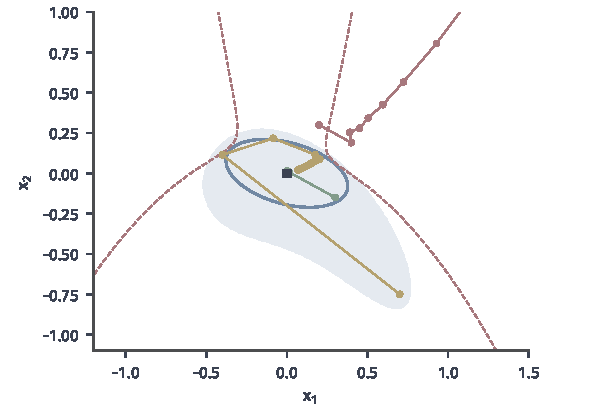
\includegraphics[width=100mm]{figures/03-optimization-evolution-and-signals/02-processes-and-trajectory-evolution/matplotlib/dds-basin-estimate/figure.pdf}
  \caption{子水平集给出的吸引区域。映射$F(x_1,x_2)=(0.5x_1+x_2,\,0.5x_2+x_1^2)$，$V=\bm x^{\top}\bm P\bm x$沿用图~\ref{fig:dds-lyapunov-ellipses}的$\bm P$。浅蓝区域是数值估计的吸引域（$700\times560$网格，迭代$200$步后距原点小于$10^{-6}$）；红色虚线是$\Delta V=0$的曲线；蓝色椭圆$\Omega_c$（$c=0.164$）完全落在$\Delta V<0$的一侧。绿色轨道从椭圆内出发；黄色轨道从椭圆外、吸引域内出发，也收敛；红色轨道从吸引域外出发并逃逸。}
  \label{fig:dds-basin-estimate}
\end{figure}

图~\ref{fig:dds-basin-estimate}把证明得到的椭圆和数值估计的真实吸引域画在一起。椭圆是一个保守的估计：吸引域在右下方伸得更远，黄色轨道从椭圆外出发同样收敛，只是这一点没有被这个$V$证明。估计的大小取决于$V$的选择，换一个$\bm Q$或者非二次的$V$可能证出更大的区域。$c^*$本身是网格上的数值估计；严格的证明需要在$\Omega_c$上对$\Delta V<0$给出解析或区间算术的验证，网格检查只是提示。

\paragraph{非严格下降}
若只知道$\Delta V\leq0$，定理只保证稳定，不保证收敛。旋转$\bm x_{n+1}=\bm R(\varphi)\bm x_n$取$V=\lVert\bm x\rVert_2^2$，$\Delta V\equiv0$，非零初值的轨道永远在圆周上转动。能量不增加，不等于能量会耗尽。但非严格下降仍然提供了信息：轨道最终只能停留在不再下降的地方。

\begin{theorem}[非严格下降时的极限点]
\label{thm:dds-lasalle}
设$\Omega\subseteq\mathbb R^d$紧且正向不变，$F$在$\Omega$上连续，$V:\Omega\to\mathbb R$连续，且$\Delta V(\bm x)\leq0$对一切$\bm x\in\Omega$成立。记$E=\{\bm x\in\Omega:\Delta V(\bm x)=0\}$。则对任意$\bm x_0\in\Omega$，轨道的每个极限点$\bm z$都满足：$F^k(\bm z)\in E$对全部$k\geq0$成立。特别地，若$E$中唯一一个整条正向轨道都留在$E$内的点是平衡点$\bm x_*$，则$\bm x_n\to\bm x_*$。
\end{theorem}

\begin{proof}
$V(\bm x_n)$单调不增，又因$V$在紧集上有下界而收敛到某个$c$。设子列$\bm x_{n_j}\to\bm z$。对固定的$k$，$F^k$连续，所以$\bm x_{n_j+k}=F^k(\bm x_{n_j})\to F^k(\bm z)$，从而$V(F^k(\bm z))=\lim_jV(\bm x_{n_j+k})=c$。这对每个$k$成立，于是$\Delta V(F^k(\bm z))=V(F^{k+1}(\bm z))-V(F^k(\bm z))=0$，即$F^k(\bm z)\in E$。最后一句：在所述条件下每个极限点都等于$\bm x_*$；若$\bm x_n\not\to\bm x_*$，在紧集$\Omega$中可以取出一个离$\bm x_*$至少$\varepsilon$的收敛子列，其极限是不等于$\bm x_*$的极限点，矛盾。
\end{proof}

这个结论是LaSalle不变性原理的离散形式，第~\ref{sec:dds-limit-sets}小节引入极限集合后还会用更紧凑的语言重述它。看一个例子：$F(\bm x)=\bm R(\varphi)\bm D\bm x$，$\bm D=\operatorname{diag}(1,1/2)$，即先把第二坐标减半、再旋转$\varphi$。取$V=\lVert\bm x\rVert_2^2$，旋转不改变长度，所以
\[
  \Delta V(\bm x)=\lVert\bm D\bm x\rVert_2^2-\lVert\bm x\rVert_2^2=-\tfrac34x_2^2\leq0 .
\]
$V$只在第二坐标上耗散，$E$是整条横轴$\{x_2=0\}$，比平衡点大得多。但横轴上的点$(z_1,0)$一步后到达$z_1(\cos\varphi,\sin\varphi)$，只要$\sin\varphi\neq0$且$z_1\neq0$，它就离开了横轴。所以整条轨道都留在$E$中的点只有原点，任何闭球都是紧的正向不变集，由定理全部轨道收敛到原点。旋转把横轴上的“能量”不断转到会耗散的方向，这正是非严格下降仍能导致收敛的机制。反之，$\varphi=0$时$F=\bm D$，横轴上每个点都是平衡点，轨道$\bm x_n=(x_{0,1},2^{-n}x_{0,2})$收敛到横轴上的某一点，而不是原点。

% 第1章第4节：非线性轨道的长期行为（极限集合与吸引子；参数变化与分岔；敏感依赖与有限精度）。

\section{非线性轨道的长期行为}
\label{sec:dds-nonlinear-long-term}

上一节的判据围绕一个平衡点展开：轨道会不会回到它。非线性系统的长期行为丰富得多。轨道可能被一条周期轨道吸引而永不停下，不同初值可能去往不同的终点，参数稍作改变，终点的数目和稳定性也可能突然改变；还有些轨道始终有界，却既不收敛也不周期，近邻的两条轨道以指数速度分开。本节保持同一个问题——“轨道最终到哪里，结论如何随参数和初值改变”——依次讨论描述终点的极限集合、参数变化引起的分岔，以及敏感依赖对有限精度计算的影响。

\subsection{极限集合与吸引子}
\label{sec:dds-limit-sets}

\paragraph{有界而不收敛的轨道}
$r=3.2$时，Logistic映射的轨道趋向周期二轨道$\{x_-,x_+\}$。序列$x_n$本身没有极限，它的偶数项和奇数项却分别收敛到$x_-$与$x_+$（或者相反）。要描述这样的长期行为，“极限”需要从一个点推广为一个集合：收集轨道在越来越晚的时刻反复靠近的所有点。

\begin{definition}[$\omega$极限集]
\label{def:dds-omega-limit}
设$X\subseteq\mathbb R^d$，$F:X\to X$，$\bm x_0\in X$，$\bm x_n=F^n(\bm x_0)$。称
\[
  \omega(\bm x_0)=\bigl\{\bm z\in\mathbb R^d:\text{存在}\ n_j\to\infty\ \text{使}\ \bm x_{n_j}\to\bm z\bigr\}
\]
为$\bm x_0$的\term{$\omega$极限集}（$\omega$-limit set），即轨道全部子列极限组成的集合。
\end{definition}

等价地，$\omega(\bm x_0)=\bigcap_{N\geq0}\overline{\{\bm x_n:n\geq N\}}$：一个点属于极限集，当且仅当轨道无论多晚都还会回到它的任意邻域。几个例子显示了极限集的不同形态。轨道收敛到$\bm x_*$时，$\omega(\bm x_0)=\{\bm x_*\}$。上面的Logistic轨道有$\omega(x_0)=\{x_-,x_+\}$。$x_{n+1}=x_n+1$的轨道趋于无穷，没有任何收敛子列，$\omega(x_0)=\varnothing$。

极限集也可以是一整条曲线。把单位圆上的点记为角度$\theta\in[0,1)$（以整圈为单位），考察转动$\theta_{n+1}=\theta_n+\alpha\pmod1$。若$\alpha=p/q$是有理数，每条轨道都是周期$q$的轨道。若$\alpha$是无理数，轨道在圆上稠密，从而$\omega(\theta_0)$是整个圆。证明只用抽屉原理：$\alpha$无理时各点$\theta_n=\theta_0+n\alpha\pmod1$两两不同；任取正整数$N$，前$N+1$个点中必有两个相距小于$1/N$，设为$\theta_i,\theta_j$（$i<j$），则转动$k=j-i$步相当于沿圆周移动一个非零的距离$\beta<1/N$。从任意$\theta_m$开始，每$k$步前进$\beta$，所以轨道的后段以小于$1/N$的间隔走遍整个圆，圆上每个长度为$1/N$的弧都会被无限次访问。$N$任意，即得结论。这条轨道既不收敛也不周期，却在长期中均匀地扫过一个集合。

\paragraph{极限集合的基本性质}
极限集在什么条件下可以作为“轨道的终点”使用？至少需要它非空，并且轨道真的趋近它。下面的定理说明，轨道停留在一个紧集中时这两点都成立，而且极限集本身是不变集。

\begin{theorem}[$\omega$极限集的性质]
\label{thm:dds-omega-limit-properties}
设$X\subseteq\mathbb R^d$为闭集，$F:X\to X$连续，$\bm x_0\in X$的轨道包含在某个紧集$K\subseteq X$中。则$\omega(\bm x_0)$非空、紧，满足$F(\omega(\bm x_0))=\omega(\bm x_0)$，并且
\[
  \operatorname{dist}\bigl(\bm x_n,\omega(\bm x_0)\bigr)\to0\qquad(n\to\infty).
\]
\end{theorem}

\begin{proof}
记$\omega=\omega(\bm x_0)$。由Bolzano--Weierstrass定理，$K$中的序列$(\bm x_n)$有收敛子列，故$\omega\neq\varnothing$，且$\omega\subseteq K$。$\omega$是闭集$\overline{\{\bm x_n:n\geq N\}}$的交，因而闭；作为紧集$K$的闭子集，它是紧集。

正向不变：若$\bm x_{n_j}\to\bm z$，由连续性$\bm x_{n_j+1}=F(\bm x_{n_j})\to F(\bm z)$，所以$F(\bm z)\in\omega$。反向包含：设$\bm x_{n_j}\to\bm z$，序列$(\bm x_{n_j-1})$在$K$中，有子列收敛到某个$\bm w\in\omega$，沿这一子列$F(\bm x_{n_j-1})=\bm x_{n_j}\to\bm z$，故$F(\bm w)=\bm z$。于是$\omega\subseteq F(\omega)$。

趋近：若结论不成立，存在$\varepsilon>0$与$n_j\to\infty$使$\operatorname{dist}(\bm x_{n_j},\omega)\geq\varepsilon$。在$K$中取其收敛子列，极限属于$\omega$，与距离至少为$\varepsilon$矛盾。
\end{proof}

紧性不可省略：$x_{n+1}=x_n+1$满足其余所有条件，极限集却是空集。有了这个定理，第~\ref{sec:dds-lyapunov}小节非严格下降的结论可以说得更紧凑。在定理~\ref{thm:dds-lasalle}的条件下，$\omega(\bm x_0)$是不变集，并且其中每一点的整条正向轨道都留在$E$中；所以$\omega(\bm x_0)$包含于$E$的最大不变子集$M$，轨道趋近$M$。这就是离散时间的\term{LaSalle不变性原理}（LaSalle invariance principle）。

\paragraph{吸引子与吸引域}
有了极限集，就可以谈论“一群初值共同的终点”。文献中吸引子的定义并不统一，有的还要求稳定性或不可再分；本章采用下面的版本，并在使用时注明。

\begin{definition}[吸引子与吸引域]
\label{def:dds-attractor}
设$F:X\to X$连续，$A\subseteq X$为非空紧集且$F(A)=A$。若存在包含$A$的开集$W$，使每个$\bm x_0\in W$满足$\operatorname{dist}(F^n(\bm x_0),A)\to0$，称$A$为\term{吸引子}（attractor）。集合
\[
  \mathcal B(A)=\{\bm x_0\in X:\operatorname{dist}(F^n(\bm x_0),A)\to0\}
\]
称为$A$的\term{吸引域}（basin of attraction）。
\end{definition}

渐近稳定的平衡点$\{\bm x_*\}$与稳定的周期轨道都是吸引子。吸引域通常比证明得到的子水平集大得多（图~\ref{fig:dds-basin-estimate}），但它有一个可以直接证明的性质：若$\bm x_*$渐近稳定、$F$在$X=\mathbb R^d$上连续，则$\mathcal B(\{\bm x_*\})$是开集。事实上，取吸引半径$r$，若$\bm x_0\in\mathcal B$，则某个$F^m(\bm x_0)$落在开球$B_r(\bm x_*)$中；$F^m$连续，所以$\bm x_0$的一个邻域也被$F^m$送进$B_r(\bm x_*)$，这个邻域中的每一点随后都收敛到$\bm x_*$。

同一个系统可以有几个吸引子，它们的吸引域把空间分成几块。图~\ref{fig:dds-newton-basins}画出用牛顿法求$z^3=1$的复根时的情形。迭代$N(z)=z-(z^3-1)/(3z^2)=(2z^3+1)/(3z^2)$以三个立方根$1,\mathrm e^{\pm2\pi\mathrm i/3}$为平衡点。由$N'(z)=2(z^3-1)/(3z^3)$，三个根处$N'=0$，线性化给出极强的局部吸引，靠近根之后误差大致每步平方一次。可是远离根时，初值去往哪个根并不显然：图中按60步后到达的根给每个初值着色，三块颜色在交界处以越来越细的尺度反复交错。

\begin{figure}[htbp]
  \centering
  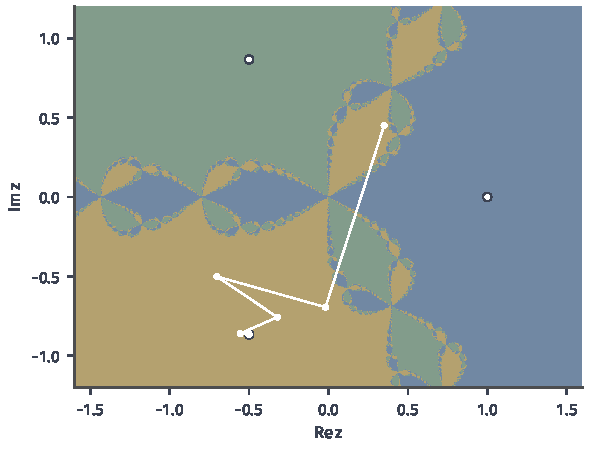
\includegraphics[width=100mm]{figures/03-optimization-evolution-and-signals/02-processes-and-trajectory-evolution/matplotlib/dds-newton-basins/figure.pdf}
  \caption{牛顿法求$z^3=1$的三个吸引域。复平面$[-1.6,1.6]\times[-1.2,1.2]$上$900\times675$个初值各迭代$N(z)=(2z^3+1)/(3z^2)$六十步，按到达的根着色：蓝色趋于$1$，绿色趋于$\mathrm e^{2\pi\mathrm i/3}$，黄色趋于$\mathrm e^{-2\pi\mathrm i/3}$；白圈为三个根。白色折线是从$0.35+0.45\mathrm i$出发的一条轨道，它先跳过原点附近，最后落入左下方的根。}
  \label{fig:dds-newton-basins}
\end{figure}

这张图同时说明了数值图像的边界。每个像素只代表一个初值的有限步计算，着色依赖迭代步数和判定容差；它提示吸引域的边界非常复杂，却不能证明边界的结构。复动力系统的理论确实证明了，这三个吸引域有共同的边界，边界上任一点附近三种颜色都会出现，但这一结论需要专门的工具，本章不证。读图时应把它当作观察，而不是定理。

一维的Logistic映射也有类似的问题，只是简单得多。$r=3.2$时，周期二轨道吸引了$(0,1)$中除可数个点以外的全部初值；这一结论需要一维映射的专门理论，这里只说明例外点为何至多可数。例外的是最终恰好落在不稳定平衡点$0$或$x_r=0.6875$上的点，例如$x_0=0.3125$满足$F(0.3125)=0.6875$。每个点在$F$下至多有两个前像，所以这些例外点可以按“几步之后落到平衡点”逐层列出，组成一个可数集。

\subsection{参数变化与分岔}
\label{sec:dds-bifurcation}

\paragraph{沿参数跟踪平衡点}
模型几乎总含参数：Logistic映射的$r$，梯度下降的步长，动量迭代的$\beta$。参数连续变化时，平衡点会不会也连续变化，稳定性会不会保持？考察一族一维映射$F_\mu(x)$，$\mu$为实参数，平衡点满足$G(x,\mu)=F_\mu(x)-x=0$。若$(x_*,\mu_0)$是一个平衡点，$F$连续可微，且
\[
  \partial_xG(x_*,\mu_0)=F_{\mu_0}'(x_*)-1\neq0,
\]
则由隐函数定理，在$\mu_0$附近存在唯一的连续可微函数$x_*(\mu)$，使$x_*(\mu)$是$F_\mu$在$x_*$附近唯一的平衡点。导数$F_\mu'(x_*(\mu))$随$\mu$连续变化，只要它不穿过$\pm1$，线性化判据给出的稳定性就保持不变。

所以平衡点的数目或稳定性只可能在$F'=1$或$F'=-1$处改变。参数经过某个值时，平衡点或周期轨道的数目、稳定性发生改变，这种现象称为\term{分岔}（bifurcation），这个参数值称为分岔点。$F'=1$时隐函数定理失效，平衡点可能成对出现或消失；$F'=-1$时平衡点本身仍可延续，但两步映射$F^2$的导数$(F')^2=1$，周期二轨道可能从这里分出。下面两个例子分别对应这两种情形。

\paragraph{鞍结分岔}
考察$F_\mu(x)=x+\mu-x^2$。平衡点方程$x=x+\mu-x^2$即$x^2=\mu$。$\mu<0$时没有平衡点，并且$x_{n+1}-x_n=\mu-x_n^2<0$，每条轨道都严格递减，最终趋于$-\infty$。$\mu>0$时有两个平衡点$\pm\sqrt\mu$。由$F_\mu'(x)=1-2x$，在$\sqrt\mu$处导数为$1-2\sqrt\mu$，当$0<\mu<1$时落在$(-1,1)$内，该点指数稳定；在$-\sqrt\mu$处导数为$1+2\sqrt\mu>1$，该点不稳定。$\mu=0$时两者合并为$x=0$，导数恰好为$1$。图~\ref{fig:dds-bifurcation-branches}(a)画出这两条分支：参数从负到正穿过$0$时，一对平衡点“凭空”出现，一稳一不稳。这种分岔称为\term{鞍结分岔}（saddle-node bifurcation）。

\begin{figure}[htbp]
  \centering
  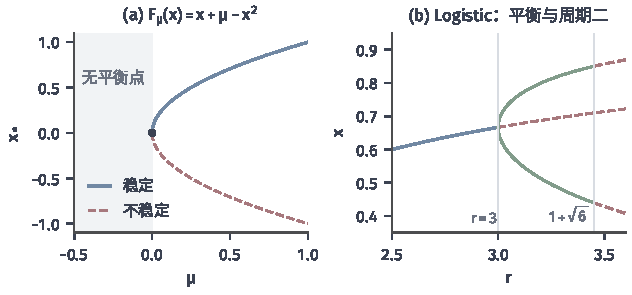
\includegraphics[width=107mm]{figures/03-optimization-evolution-and-signals/02-processes-and-trajectory-evolution/matplotlib/dds-bifurcation-branches/figure.pdf}
  \caption{两类分岔的解析分支，实线稳定、虚线不稳定。(a)$F_\mu(x)=x+\mu-x^2$的平衡点$\pm\sqrt\mu$；$\mu<0$（灰色区域）没有平衡点，$\mu=0$处两点合并，图中只画到$\mu=1$，此后$\sqrt\mu$处的导数将低于$-1$。(b)Logistic映射：平衡点$x_r=1-1/r$在$r<3$时稳定（蓝），$r>3$时失稳（红虚线）；周期二轨道$x_\pm$从$r=3$分出，在$3<r<1+\sqrt6$时稳定（绿），此后失稳。}
  \label{fig:dds-bifurcation-branches}
\end{figure}

\paragraph{倍周期分岔：Logistic映射的可解析区间}
Logistic映射在$r\in[0,4]$上把$[0,1]$映回自身，前面已经算出它的平衡点和周期二轨道，现在把这些结果按参数排起来。$0\leq r<1$时，$F_r'(0)=r<1$，原点指数稳定，$x_r=1-1/r$不在$[0,1]$中。$r$越过$1$，$x_r$进入$[0,1]$并接管稳定性：$F_r'(0)=r>1$使原点失稳，$F_r'(x_r)=2-r\in(-1,1)$对$1<r<3$成立。

$r=3$时$F_r'(x_r)=-1$。越过$3$以后，$x_r$不稳定，而式子$x_\pm=\bigl((r+1)\pm\sqrt{(r+1)(r-3)}\bigr)/(2r)$给出的周期二轨道恰好在此时出现。它的乘子是$-r^2+2r+4$：$r=3$时等于$1$，随$r$增大而减小，在$r=1+\sqrt6\approx3.449$时降到$-1$。所以$3<r<1+\sqrt6$时，周期二轨道是吸引子（图~\ref{fig:dds-bifurcation-branches}(b)）。图~\ref{fig:dds-period-two-graph}给出了几何画面：$F'(x_r)$穿过$-1$时，$F^2$在$x_r$处的斜率$(F'(x_r))^2$由小于$1$变为大于$1$，$F^2$的图像在$x_r$两侧各多穿过对角线一次，多出的两个交点就是$x_\pm$。导数穿过$-1$时，周期翻倍的轨道从原平衡点分出，原平衡点同时失稳，这称为\term{倍周期分岔}（period-doubling bifurcation）。

同样的机制出现在优化里，这时分岔参数是步长。梯度下降在最小点处的线性化导数是$1-\eta f''(x_*)$，步长增大使它穿过$-1$，迭代就从收敛变为在最小点两侧来回跳动。

\begin{example}[步长引起的倍周期分岔]
\label{ex:dds-step-size-bifurcation}
对$f(x)=x^4/4-x^2/2$作梯度下降，$F_\eta(x)=x-\eta(x^3-x)$，步长$\eta>0$。平衡点是$f$的驻点$0,\pm1$。$F_\eta'(x)=1-\eta(3x^2-1)$，在局部极大点$0$处为$1+\eta>1$，不稳定；在两个最小点处为$1-2\eta$，所以$0<\eta<1$时最小点指数稳定，$\eta=1$时导数恰为$-1$。临界步长$\eta=1$正是$2/f''(\pm1)$，与二次目标上的步长条件一致。越过$1$以后，从$x_0=1.2$出发迭代$2000$步的数值结果显示：$\eta=1.05$时轨道趋于周期二轨道$\{0.873,1.091\}$，$\eta=1.1$时为$\{0.815,1.116\}$，乘子分别约为$0.60$和$0.18$，都是稳定的；$\eta=1.2$时乘子约为$-0.68$，仍然稳定但已接近下一次翻倍。所以步长略大于临界值时，梯度下降并不发散，而是稳定地在最小点两侧跳动，目标值不再下降到最小值；这与发散是两种不同的失败方式。
\end{example}

\paragraph{分岔图：作为观察的补充}
$r>1+\sqrt6$以后，周期二轨道的乘子小于$-1$，同样的机制作用于$F^2$，分出周期四的轨道；再往后又有周期八、十六……解析计算越来越难，数值观察成了主要手段。图~\ref{fig:dds-logistic-bifurcation}上半部分对$1500$个$r$值各自丢弃前$1000$步、画出随后$400$个状态：稳定周期轨道表现为有限个点，倍周期表现为分叉；数值计算显示，翻倍发生的参数值依次约为$3$、$3.449$、$3.544$、……，间隔越来越小，在$r\approx3.5699$附近累积。此后大部分参数下点连成一片，其间又夹着若干周期窗口，最显眼的是$r\approx3.83$附近的周期三窗口。

\begin{figure*}[htbp]
  \centering
  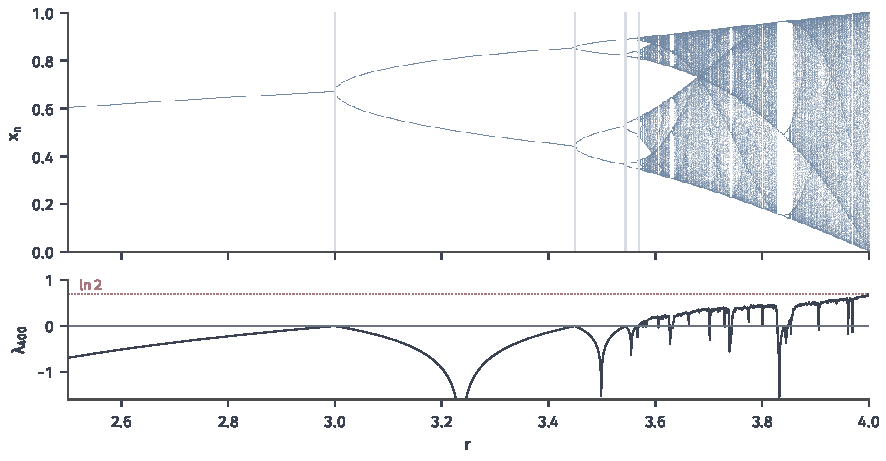
\includegraphics[width=150mm]{figures/03-optimization-evolution-and-signals/02-processes-and-trajectory-evolution/matplotlib/dds-logistic-bifurcation/figure.pdf}
  \caption{Logistic映射的分岔图与有限时间Lyapunov指数。上：对$r\in[2.5,4]$的$1500$个值，从$x_0=0.2$出发丢弃前$1000$步，画出随后$400$步的状态；竖线标出$r=3$、$1+\sqrt6$、$3.544$与累积点$3.5699$。下：同样$400$步上$\ln|F_r'(x_n)|$的平均值，零线以上表示近邻轨道平均以指数速度分离，红色点线为$\ln2$。两图都是有限步数值观察。}
  \label{fig:dds-logistic-bifurcation}
\end{figure*}

这张图容易被读得过头。点连成一片只说明有限步内轨道没有落到少数几个点上；它可能是混沌，也可能是周期很长或收敛很慢的轨道，还可能是舍入误差的产物。说某个参数下轨道“混沌”，需要证明诸如正Lyapunov指数、稠密轨道等性质，而不是看图。下一小节在$r=4$这个可以精确求解的参数上完成这样的证明。

\subsection{敏感依赖与有限精度}
\label{sec:dds-sensitivity}

\paragraph{两条近邻轨道的分离}
取$r=4$，从$x_0=0.2$和$x_0=0.2+10^{-10}$出发，用$120$位十进制精度计算两条轨道（图~\ref{fig:dds-sensitive-separation}）。前二十多步里两条轨道在图上完全重合；它们的距离却从$10^{-10}$开始，大致沿着$10^{-10}\cdot2^n$的直线增长，第$30$步超过$0.1$，此后两条轨道毫无关系。初值相差百亿分之一，三十步后的状态就无法用其中一条预测另一条，这就是\term{敏感依赖}（sensitive dependence on initial conditions）。

\begin{figure}[htbp]
  \centering
  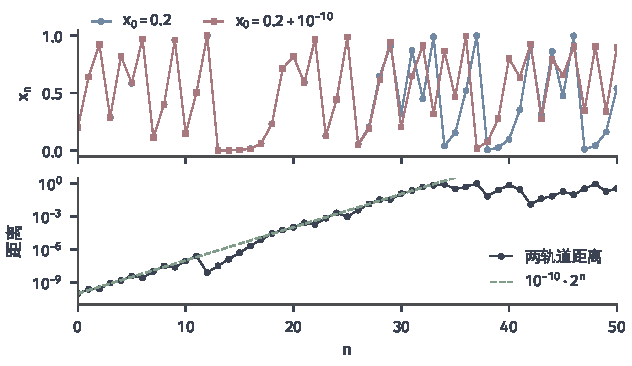
\includegraphics[width=107mm]{figures/03-optimization-evolution-and-signals/02-processes-and-trajectory-evolution/matplotlib/dds-sensitive-separation/figure.pdf}
  \caption{$r=4$时两条近邻轨道的分离。上：从$0.2$（蓝）与$0.2+10^{-10}$（红）出发的轨道，均以$120$位十进制精度计算。下：两轨道距离（对数纵轴）与参考线$10^{-10}\cdot2^n$。距离按每步约翻倍的速度增长，第$30$步超过$0.1$后在$[0,1]$的尺度上饱和；第$12$步的凹陷来自$x_{11}\approx0.504$：那里$F_4'(x)=4-8x$接近零，距离被暂时压缩，随后轨道贴近$0$，导数接近$4$，距离又迅速放大。}
  \label{fig:dds-sensitive-separation}
\end{figure}

分离速度可以用导数定量描述。设$F$可微，初值偏差$\delta$很小，则由链式法则
\[
  F^n(x_0+\delta)-F^n(x_0)\approx(F^n)'(x_0)\,\delta=\Bigl(\prod_{k=0}^{n-1}F'(x_k)\Bigr)\delta .
\]
偏差每经过一步就乘以当地的导数。把乘积取对数并平均，得到有限时间的增长率
\begin{equation}
  \lambda_n(x_0)=\frac1n\sum_{k=0}^{n-1}\ln\bigl|F'(x_k)\bigr| .
  \label{eq:dds-finite-lyapunov}
\end{equation}

\begin{definition}[Lyapunov指数]
\label{def:dds-lyapunov-exponent}
设$F$可微，且轨道$(x_k)$上$F'(x_k)\neq0$。若极限$\lambda(x_0)=\lim_{n\to\infty}\lambda_n(x_0)$存在，称为$x_0$处的\term{Lyapunov指数}（Lyapunov exponent）。
\end{definition}

指数的含义要和使用条件一起读。在稳定平衡点上，$\lambda=\ln|F'(x_*)|<0$；在乘子为$m$的稳定周期$p$轨道上，$\lambda=\frac1p\ln|m|<0$；它们都说明近邻轨道被拉拢。$\lambda>0$表示近邻轨道平均以$\mathrm e^{\lambda n}$的速度分开，但仅凭正指数不能断言轨道复杂：不稳定平衡点上也有$\lambda=\ln|F'(x_*)|>0$，而那条轨道一动不动。此外，$\lambda_n$是有限时间的量，近似式还要求偏差始终足够小；偏差长到状态空间的尺度后，线性近似就不成立了，图~\ref{fig:dds-sensitive-separation}中距离的饱和正是这个原因。图~\ref{fig:dds-logistic-bifurcation}下半部分画出了$\lambda_{400}$：周期窗口里为负，分岔点处接近$0$，连成一片的区域大多为正。

\paragraph{$r=4$时的精确解：每步翻倍的角度}
$r=4$的Logistic映射可以精确求解，敏感依赖的来源因此一目了然。令$h(\theta)=\sin^2(\pi\theta)$，则
\[
  F_4\bigl(h(\theta)\bigr)=4\sin^2(\pi\theta)\cos^2(\pi\theta)=\sin^2(2\pi\theta)=h(2\theta).
\]
所以若$x_0=h(\theta_0)$，归纳得
\begin{equation}
  x_n=\sin^2\bigl(\pi\,2^n\theta_0\bigr).
  \label{eq:dds-logistic-exact}
\end{equation}
$h$以$1$为周期，只有$\theta$的小数部分起作用；而$[0,1]$中的每个$x$都可以写成$h(\theta)$。在$\theta$坐标下，Logistic映射变成了倍角映射$\theta\mapsto2\theta\pmod1$。

把$\theta_0$写成二进制小数$0.b_1b_2b_3\ldots$，乘以$2$再取小数部分就是把各位左移一位、丢掉首位：$\theta_n=0.b_{n+1}b_{n+2}\ldots$。于是$x_n$只取决于$\theta_0$第$n+1$位以后的数字。两个初值的$\theta$若只在前$k$位一致，大约$k$步以后它们的状态就由互不相关的数字决定。初值精度每多一位二进制，可预测的步数只多一步。

指数也可以直接算出。对式$F_4\circ h=h\circ(2\,\cdot)$用链式法则$n$次，得$(F_4^n)'(h(\theta_0))\,h'(\theta_0)=2^n\,h'(\theta_n)$，其中$h'(\theta)=\pi\sin(2\pi\theta)$。在$h'(\theta_0)\neq0$（即$x_0\notin\{0,1\}$）时，
\[
  \lambda_n(x_0)=\frac1n\ln\bigl|(F_4^n)'(x_0)\bigr|=\ln2+\frac1n\ln\frac{|\sin(2\pi\theta_n)|}{|\sin(2\pi\theta_0)|}.
\]
只要轨道不越来越贴近$x=0$或$x=1$，使得$\frac1n\ln|\sin(2\pi\theta_n)|\to0$，就有$\lambda(x_0)=\ln2$；图~\ref{fig:dds-logistic-bifurcation}在$r=4$处的数值约为$0.69$，与$\ln2\approx0.693$相符。例外的轨道确实存在：$x_0=3/4$是平衡点，$F_4'(3/4)=-2$，指数恰为$\ln2$；$x_0=0$是平衡点，$F_4'(0)=4$，指数为$\ln4$；$x_0=1/2$两步后落到$0$并停住。所以“指数为$\ln2$”是对一类轨道的结论，不是对每个初值都成立。

\paragraph{有限精度：每步丢失一个比特}
敏感依赖立刻影响数值计算。双精度浮点数有$53$位二进制有效数字，单精度有$24$位。用浮点数计算$r=4$的轨道，每一步的舍入误差约为$10^{-16}$（双精度）量级，随后按每步约翻倍的速度放大。图~\ref{fig:dds-rounding-divergence}比较两种精度与$120$位十进制参考值：单精度轨道在第$23$步误差超过$0.1$，双精度在第$52$步超过$0.1$，几乎恰好是有效位数。之后算出的数仍在$[0,1]$中，看上去正常，但与从$0.2$出发的真实轨道已经没有关系。

\begin{figure}[htbp]
  \centering
  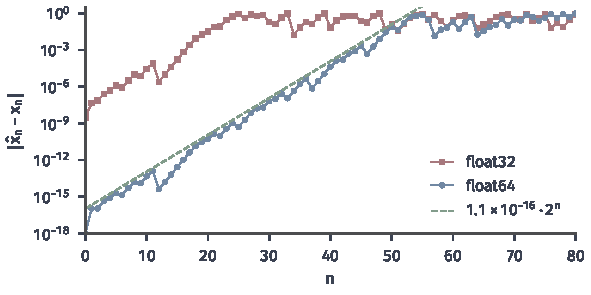
\includegraphics[width=100mm]{figures/03-optimization-evolution-and-signals/02-processes-and-trajectory-evolution/matplotlib/dds-rounding-divergence/figure.pdf}
  \caption{有限精度下$r=4$轨道的偏离。$x_0=0.2$，分别用单精度（红）与双精度（蓝）逐步计算，与$120$位十进制参考轨道比较，纵轴取对数，绿色虚线为$1.1\times10^{-16}\cdot2^n$。双精度第$0$步的误差来自$0.2$本身不能用二进制精确表示；两种精度分别在第$23$、$52$步误差超过$0.1$。}
  \label{fig:dds-rounding-divergence}
\end{figure}

这不是程序错误，而是映射本身的性质：再好的算法也不能在每步翻倍的误差面前长期保持逐点精度。提高精度只能线性地延长可预测步数，每多一位十进制数字大约多$\log_210\approx3.3$步。另一方面，逐点预测失效并不意味着一切长期陈述都失去意义。轨道在$[0,1]$中各处停留的频率、时间平均等统计性质，往往对这种误差不敏感；对某些满足专门条件的系统，还能证明计算出的轨道整段贴近另一条真实轨道。本章只建立“轨道误差”的含义，统计规律和概率描述留给第~\ref{chap:discrete-time-stochastic-processes}章。

% 第1章第5节：轨迹计算中的误差传播（初值与逐步计算误差；输入与模型扰动）。

\section{轨迹计算中的误差传播}
\label{sec:dds-error-propagation}

上一节看到，有限精度可以让$r=4$的Logistic轨道在五十步内完全失真。本节把这种现象放进一般框架：离散模型已经给定，我们实际算出的序列与模型的真实轨道相差多少？误差有几个来源：初值不准，每一步计算带有残差，输入与设定值有偏差，模型本身与要描述的过程有出入。它们注入的位置不同，却都要经过此后的动力学传播。

需要说明比较的对象。这里递推本身就是模型，我们问的是“这个递推算得多准”。第~\ref{chap:ordinary-differential-equations}章用离散步长逼近常微分方程时，递推是对另一个连续对象的近似，误差还包括每步的截断误差，即离散公式与连续演化之差。两种误差在数学上可以用同一个累计不等式处理，但来源和随步长变化的方式不同，不应混为一谈。

\subsection{初值与逐步计算误差}
\label{sec:dds-computation-error}

\paragraph{把计算误差写成每步残差}
设模型为$\bm x_{n+1}=F(\bm x_n)$，实际算出的序列为$\hat{\bm x}_n$。无论误差来自舍入、内层迭代没有完全收敛，还是用查表或低精度近似代替了$F$，都可以统一写成
\[
  \hat{\bm x}_{n+1}=F(\hat{\bm x}_n)+\bm r_n ,
\]
其中$\bm r_n$是第$n$步的残差：把上一步的计算值代入模型，与本步计算值的差。记误差$\bm e_n=\hat{\bm x}_n-\bm x_n$。若$F$在某个区域$D$上满足$\lVert F(\bm x)-F(\bm y)\rVert\leq L\lVert\bm x-\bm y\rVert$，且两条序列都在$D$中，则
\[
  \lVert\bm e_{n+1}\rVert\leq\lVert F(\hat{\bm x}_n)-F(\bm x_n)\rVert+\lVert\bm r_n\rVert\leq L\lVert\bm e_n\rVert+\lVert\bm r_n\rVert .
\]
误差满足一个“乘以$L$、再加新残差”的标量不等式。它的解与第~\ref{sec:dds-constant-coefficient}小节的仿射递推有同样的结构。

\begin{lemma}[离散Grönwall不等式]
\label{lem:dds-discrete-gronwall}
设非负数列$(a_n)$、$(b_n)$、$(L_n)$满足$a_{n+1}\leq L_na_n+b_n$，$n\geq0$。则
\[
  a_n\leq\Bigl(\prod_{k=0}^{n-1}L_k\Bigr)a_0+\sum_{k=0}^{n-1}\Bigl(\prod_{i=k+1}^{n-1}L_i\Bigr)b_k ,
\]
空乘积取$1$。特别地，$L_n\equiv L$时$a_n\leq L^na_0+\sum_{k=0}^{n-1}L^{\,n-1-k}b_k$。
\end{lemma}

\begin{proof}
$n=0$时右边为$a_0$。若对$n$成立，则因$L_n\geq0$，
\[
  a_{n+1}\leq L_na_n+b_n\leq\Bigl(\prod_{k=0}^{n}L_k\Bigr)a_0+\sum_{k=0}^{n-1}\Bigl(\prod_{i=k+1}^{n}L_i\Bigr)b_k+b_n ,
\]
最后一项正是$k=n$时的求和项。
\end{proof}

引理与递推解~\eqref{eq:dds-variation-constants}一一对应：初始误差像初态一样被逐步放大或缩小，每步残差像输入一样在注入后继续传播。只是这里用不等式代替了等式，用Lipschitz常数代替了矩阵。

\begin{theorem}[逐步计算误差的传播界]
\label{thm:dds-error-propagation}
设$D\subseteq\mathbb R^d$，$F:D\to\mathbb R^d$在$D$上$L$-Lipschitz。设模型轨道$\bm x_{n+1}=F(\bm x_n)$与计算序列$\hat{\bm x}_{n+1}=F(\hat{\bm x}_n)+\bm r_n$在$0\leq n\leq N$时都位于$D$中，且$\lVert\bm r_n\rVert\leq\eta$。则对$0\leq n\leq N$，
\begin{equation}
  \lVert\hat{\bm x}_n-\bm x_n\rVert\leq L^n\lVert\hat{\bm x}_0-\bm x_0\rVert+\eta\sum_{k=0}^{n-1}L^k
  =\begin{cases}
    L^n\lVert\hat{\bm x}_0-\bm x_0\rVert+\eta\dfrac{L^n-1}{L-1},&L\neq1,\\[1ex]
    \lVert\hat{\bm x}_0-\bm x_0\rVert+n\eta,&L=1.
  \end{cases}
  \label{eq:dds-error-propagation}
\end{equation}
\end{theorem}

\begin{proof}
前面已得$\lVert\bm e_{n+1}\rVert\leq L\lVert\bm e_n\rVert+\eta$，对$a_n=\lVert\bm e_n\rVert$、$L_n=L$、$b_n=\eta$用引理~\ref{lem:dds-discrete-gronwall}。
\end{proof}

上界分成三种情形，对应三种截然不同的计算体验。$L<1$时，初始误差几何衰减，残差的累计被几何级数封顶，$\limsup_n\lVert\bm e_n\rVert\leq\eta/(1-L)$：误差不会越积越多。$L=1$时，残差线性累计，长时间计算的误差随步数增长。$L>1$时，误差可能按$L^n$增长，有限时间内可控，长时间则无界。定理的前提“两条序列都在$D$中”需要单独核实：若误差把计算序列推出了Lipschitz估计成立的区域，上界就不再适用，这在$L>1$时尤其要注意。

图~\ref{fig:dds-error-bound}用两个例子对比上界与实际误差。(a)中$F=\cos$，初值误差$0.1$，每步人为加入幅度不超过$\eta=10^{-3}$的残差；轨道在$[0,1.01]$中，取$L=0.85\geq\sin1.01$。实际误差很快降到$10^{-3}$量级并在其中起伏，上界从$0.1$平滑地降到$\eta/(1-L)\approx6.7\times10^{-3}$，始终在实际误差之上。(b)中$F(x)=4x(1-x)$用双精度计算，每步舍入残差不超过$2^{-52}\approx2.2\times10^{-16}$，$[0,1]$上的Lipschitz常数是$\max|F'|=4$。上界按$4^n$增长，实际误差却大致按$2^n$增长。

\begin{figure}[htbp]
  \centering
  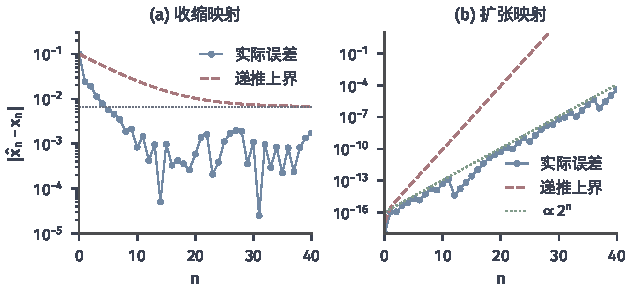
\includegraphics[width=107mm]{figures/03-optimization-evolution-and-signals/02-processes-and-trajectory-evolution/matplotlib/dds-error-bound/figure.pdf}
  \caption{递推误差上界与实际误差，纵轴取对数。(a)收缩映射$\cos x$：真实轨道从$0.2$出发，计算序列从$0.3$出发且每步加入幅度在$[\eta/2,\eta]$、符号随机（固定种子）的残差，$\eta=10^{-3}$；红色虚线为式~\eqref{eq:dds-error-propagation}取$L=0.85$的上界，点线为其极限$\eta/(1-L)$。(b)扩张映射$4x(1-x)$：双精度计算与$120$位参考轨道之差，上界取$L=4$、每步残差$2^{-52}$，并计入$0.2$的初始表示误差；绿色点线示意$2^n$的增长。}
  \label{fig:dds-error-bound}
\end{figure}

(b)中的差距说明了Lipschitz上界的保守之处。$L=4$是$|F'|$在整个区间上的最大值，只在$x=0$与$x=1$附近取到；一条典型轨道各处都要经过，它感受到的是沿轨道导数的几何平均，即第~\ref{sec:dds-sensitivity}小节的Lyapunov指数$\ln2$。若把引理中的常数$L$换成沿轨道的局部放大因子$L_k\approx|F'(x_k)|$，就能得到贴近实际的估计，代价是这些因子依赖具体轨道，事先不知道。

\paragraph{收缩更新的长期残差界}
收缩情形最值得在实际计算中利用。设$F$在完备的正向不变集$D$上是$L$-压缩（$L<1$），不动点为$\bm x_*$。以$\bm x_0=\bm x_*$为模型轨道代入定理~\ref{thm:dds-error-propagation}（仍需假设计算序列留在$D$中），得到
\[
  \lVert\hat{\bm x}_n-\bm x_*\rVert\leq L^n\lVert\hat{\bm x}_0-\bm x_*\rVert+\frac{\eta}{1-L}.
\]
无论迭代多久，计算精度都被$\eta/(1-L)$兜住；反过来，要把不动点算到精度$\varepsilon$，每步残差必须小于$(1-L)\varepsilon$。$L$越接近$1$，收缩越弱，对每步精度的要求越苛刻，这是压缩映射的一种“条件数”。

事后估计用已经算出的量判断离不动点有多远。由$\hat{\bm x}_n-\bm x_*=(\hat{\bm x}_n-F(\hat{\bm x}_n))+(F(\hat{\bm x}_n)-F(\bm x_*))$与三角不等式，
\[
  \lVert\hat{\bm x}_n-\bm x_*\rVert\leq\lVert F(\hat{\bm x}_n)-\hat{\bm x}_n\rVert+L\lVert\hat{\bm x}_n-\bm x_*\rVert ,
\]
移项后再用$F(\hat{\bm x}_n)=\hat{\bm x}_{n+1}-\bm r_n$，
\begin{equation}
  \lVert\hat{\bm x}_n-\bm x_*\rVert\leq\frac{\lVert F(\hat{\bm x}_n)-\hat{\bm x}_n\rVert}{1-L}\leq\frac{\lVert\hat{\bm x}_{n+1}-\hat{\bm x}_n\rVert+\eta}{1-L}.
  \label{eq:dds-a-posteriori}
\end{equation}
所以“相邻两步很接近就停止”在收缩映射下是有依据的，但要乘上因子$1/(1-L)$，还要计入残差$\eta$：步长小于$10^{-8}$、$L=0.99$时，离不动点的距离只能保证小于约$10^{-6}$。

\paragraph{相邻两步很近不等于接近极限}
没有收缩条件，步长小就说明不了什么。$x_{n+1}=x_n+1/x_n$从$x_0=1$出发，第$10^4$步的步长约为$0.007$，第$10^5$步约为$0.0022$，越来越小，轨道却按$\sqrt{2n}$的速度趋于无穷：步长趋于零，序列不收敛。即使序列确实收敛，步长也可能严重低估距离。回到$x_{n+1}=x_n-x_n^3$，$x_0=0.5$时第$1000$步的步长$x_n^3\approx1.1\times10^{-5}$，离极限$0$的距离却是$0.022$，是步长的两千倍。原因是原点处导数为$1$，收缩因子趋于$1$，式~\eqref{eq:dds-a-posteriori}中的$1/(1-L)$趋于无穷。判断“已经接近极限”需要动力学条件与残差一起提供依据。

\paragraph{不稳定更新放大微小残差}
误差放大最直观的例子，是试图沿着不稳定的平衡点做长时间计算。

\begin{example}[从不稳定平衡点出发的浮点计算]
\label{ex:dds-unstable-fixed-point}
取$r=3.3$的Logistic映射，平衡点$x_r=1-1/3.3=0.69\overline{69}$，这里$F'(x_r)=2-3.3=-1.3$，平衡点不稳定。把双精度下最接近$x_r$的数作为初值，第一步的残差只有约$2.2\times10^{-16}$，此后偏差每步约乘以$1.3$：第$50$步约$10^{-10}$，第$100$步约$5\times10^{-5}$，第$131$步超过$0.1$，计算序列离开平衡点，转向稳定的周期二轨道。模型轨道一动不动，计算轨道却在一百多步后面目全非。在不稳定的方向上，再小的残差也会被持续放大，这与上一节$r=4$的现象同源。
\end{example}

\subsection{输入与模型扰动}
\label{sec:dds-input-model-perturbation}

\paragraph{线性系统中的输入扰动}
初值误差只在开始时注入一次，输入误差却可能在每一步都注入。设两组初值和输入$(\bm x_0,\bm u)$与$(\tilde{\bm x}_0,\tilde{\bm u})$驱动同一个系统$\bm x_{n+1}=\bm A\bm x_n+\bm B\bm u_n$。两条轨道之差$\bm\delta_n=\bm x_n-\tilde{\bm x}_n$满足同一个线性递推，输入换成$\bm u_n-\tilde{\bm u}_n$，所以由式~\eqref{eq:dds-variation-constants}，
\[
  \bm\delta_n=\bm A^n\bm\delta_0+\sum_{j=0}^{n-1}\bm A^{\,n-1-j}\bm B(\bm u_j-\tilde{\bm u}_j).
\]

\begin{theorem}[稳定线性系统的输入响应界]
\label{thm:dds-input-response}
设$\lVert\bm A^k\rVert\leq Cq^k$对全部$k\geq0$成立，$C\geq1$，$0\leq q<1$（由定理~\ref{thm:dds-spectral-stability}，$\rho(\bm A)<1$时这样的$C,q$存在）。则
\begin{equation}
  \lVert\bm\delta_n\rVert\leq Cq^n\lVert\bm\delta_0\rVert+C\lVert\bm B\rVert\sum_{j=0}^{n-1}q^{\,n-1-j}\lVert\bm u_j-\tilde{\bm u}_j\rVert .
  \label{eq:dds-input-response}
\end{equation}
特别地：
\begin{enumerate}
  \item 若$\sup_j\lVert\bm u_j-\tilde{\bm u}_j\rVert\leq U$，则$\lVert\bm\delta_n\rVert\leq Cq^n\lVert\bm\delta_0\rVert+C\lVert\bm B\rVert U/(1-q)$对全部$n$成立；
  \item 若$\lVert\bm u_j-\tilde{\bm u}_j\rVert\to0$，则$\bm\delta_n\to\bm0$。
\end{enumerate}
\end{theorem}

\begin{proof}
式~\eqref{eq:dds-input-response}由三角不等式与$\lVert\bm A^k\bm B\bm v\rVert\leq Cq^k\lVert\bm B\rVert\lVert\bm v\rVert$得到；(1)再用$\sum_{k\geq0}q^k=1/(1-q)$。对(2)，记$w_j=\lVert\bm u_j-\tilde{\bm u}_j\rVert$，它有界，设上界为$W$。给定$\varepsilon>0$，取$J$使$j\geq J$时$w_j<\varepsilon$。把求和拆成$j<J$与$j\geq J$两段：
\[
  \sum_{j=0}^{n-1}q^{\,n-1-j}w_j\leq W\sum_{j<J}q^{\,n-1-j}+\varepsilon\sum_{j\geq J}q^{\,n-1-j}\leq Wq^{\,n-J}\frac{1}{1-q}+\frac{\varepsilon}{1-q}.
\]
$n\to\infty$时第一项趋于零，所以$\limsup_n\lVert\bm\delta_n\rVert\leq C\lVert\bm B\rVert\varepsilon/(1-q)$；$\varepsilon$任意，得$\bm\delta_n\to\bm0$。
\end{proof}

定理把输入扰动的影响分成两类。有界扰动产生有界的状态偏差，偏差的大小由扰动幅度和系统的“记忆长度”$1/(1-q)$共同决定。会消失的扰动最终不留痕迹。但持续存在的扰动会留下持续的偏差，而不会因为系统稳定就消失：温度例中若加热量一直比设定值多$0.05$，由式~\eqref{eq:dds-forced-equilibrium}，平衡温差升高$0.05/(1-0.8)=0.25$。图~\ref{fig:dds-forced-response}比较了这两种扰动：初值都偏了$1$，持续偏差的轨道最终停在高出$0.25$的位置，衰减扰动（$0.3\cdot0.7^n$）的轨道则回到标称轨迹上。

\begin{figure}[htbp]
  \centering
  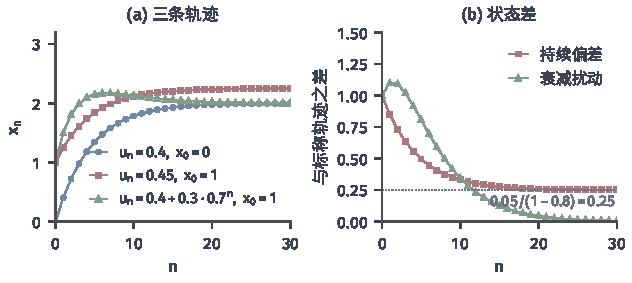
\includegraphics[width=107mm]{figures/03-optimization-evolution-and-signals/02-processes-and-trajectory-evolution/matplotlib/dds-forced-response/figure.pdf}
  \caption{持续偏差与衰减扰动。系统$x_{n+1}=0.8x_n+u_n$。(a)标称轨迹（蓝，$x_0=0$，$u_n=0.4$）、持续偏差（红，$x_0=1$，$u_n=0.45$）与衰减扰动（绿，$x_0=1$，$u_n=0.4+0.3\cdot0.7^n$）。(b)后两者与标称轨迹之差：初值差$1$按$0.8^n$消退；持续偏差留下$0.05/(1-0.8)=0.25$的稳态差（点线），衰减扰动的影响则趋于零。}
  \label{fig:dds-forced-response}
\end{figure}

稳定性是定理的必要前提。$\rho(\bm A)\geq1$时，有界输入可以产生无界状态：标量$a=1$的系统$x_n=x_0+\sum_{j<n}u_j$只是把输入累加起来，恒定的微小偏差$\delta u$也会造成线性增长的误差$n\,\delta u$。所以“初值误差会消退”与“输入误差有界”都要以稳定性为条件，而且二者分别回答不同的问题，不能用前者代替后者。

\paragraph{非线性更新中的输入与模型误差}
非线性系统没有显式解，但第~\ref{sec:dds-computation-error}小节的论证可以照搬，只需把每一步的不一致来源分开写。设真实过程按$\bm x_{n+1}=F(\bm x_n,\bm u_n)$演化，我们用另一个模型$\tilde F$和输入$\tilde{\bm u}_n$计算$\tilde{\bm x}_{n+1}=\tilde F(\tilde{\bm x}_n,\tilde{\bm u}_n)$。假设两条轨道都留在区域$D$中，并且在$D$上
\[
  \begin{gathered}
  \lVert F(\bm x,\bm u)-F(\bm y,\bm u)\rVert\leq L\lVert\bm x-\bm y\rVert,\qquad
  \lVert F(\bm x,\bm u)-F(\bm x,\bm v)\rVert\leq L_u\lVert\bm u-\bm v\rVert,\\
  \lVert F(\bm x,\bm u)-\tilde F(\bm x,\bm u)\rVert\leq\mu .
  \end{gathered}
\]
把一步差拆成三段：
\[
  \begin{aligned}
  \bm x_{n+1}-\tilde{\bm x}_{n+1}
  ={}&\bigl[F(\bm x_n,\bm u_n)-F(\tilde{\bm x}_n,\bm u_n)\bigr]
  +\bigl[F(\tilde{\bm x}_n,\bm u_n)-F(\tilde{\bm x}_n,\tilde{\bm u}_n)\bigr]\\
  &+\bigl[F(\tilde{\bm x}_n,\tilde{\bm u}_n)-\tilde F(\tilde{\bm x}_n,\tilde{\bm u}_n)\bigr],
  \end{aligned}
\]
分别对应状态差的传播、输入差和模型差。由引理~\ref{lem:dds-discrete-gronwall}，
\begin{equation}
  \lVert\bm x_n-\tilde{\bm x}_n\rVert\leq L^n\lVert\bm x_0-\tilde{\bm x}_0\rVert+\sum_{k=0}^{n-1}L^{\,n-1-k}\bigl(L_u\lVert\bm u_k-\tilde{\bm u}_k\rVert+\mu\bigr).
  \label{eq:dds-model-perturbation}
\end{equation}
三类误差来源不同，却都要经过此后的动力学传播；$L<1$时它们的累计都被几何级数封顶。

用一个数值例子说明怎样核实这些条件。

\begin{example}[线性模型代替带平方散热的温度模型]
\label{ex:dds-model-mismatch}
设房间散热还有一个与温差平方成正比的部分，真实更新为$F(x,u)=0.8x+u-0.01x^2$，而我们用线性模型$\tilde F(x,u)=0.8x+u$计算，输入都取$u_n=0.4$，初值都为$0$。先找共同的正向不变区域：在$D=[0,2]$上，$\tilde F$把$D$映到$[0.4,2]$，$F$把$D$映到$[0.4,1.96]$，都在$D$内。再算常数：$\partial_xF=0.8-0.02x\in[0.76,0.8]$，故$L=0.8$；模型差$0.01x^2\leq0.04$，故$\mu=0.04$；输入相同，第二项为零。代入式~\eqref{eq:dds-model-perturbation}，两条轨道之差不超过$0.04(1-0.8^n)/0.2<0.2$。实际上线性模型的平衡点为$2$，真实模型的平衡点满足$0.01x^2+0.2x-0.4=0$，约为$1.832$，长期差约$0.168$，确实在界内。界的大小依赖所选区域：若取更大的$D$，$\mu$会变大，界也随之变松。
\end{example}

本章到此只回答“给定的输入使状态改变了多少”。若要根据观测反过来选择输入，使状态保持在期望位置并抑制扰动的影响，就进入了控制问题，那里会把本节的输入响应界和Lyapunov函数作为设计工具重新使用。

% 第1章第6节：本章小结。

\section{本章小结}
\label{sec:dds-summary}

章首从一分钟一步的温度递推出发，问了几个问题：轨迹停在哪里，偏差会消失还是放大，非线性更新的长期结果是否同样简单，计算机算出的数字有多可信。回答这些问题时，最容易出错的地方是把不同的结论混为一谈。表~\ref{tab:dds-summary}把本章的主要结论与各自所需的条件并列：递推在每一步有定义，只保证有限轨迹可以算出；平衡点存在，只说明停在那里不会动；稳定、渐近稳定与指数稳定各有不同的量词；长期收敛还可能被瞬态放大、周期轨道或敏感依赖所取代。这些结论都不能互相替代。

\begin{table*}[htbp]
  \centering
  \begin{tabularx}{\linewidth}{>{\raggedright\arraybackslash}p{30mm}>{\raggedright\arraybackslash}X>{\raggedright\arraybackslash}p{42mm}}
    \toprule
    结论 & 所需条件 & 本章依据\\
    \midrule
    轨迹每步有定义 & 更新把状态空间映回自身，或初值位于正向不变集 & 定义~\ref{def:dds-state-model}、第~\ref{sec:dds-orbits-invariant}小节\\
    线性轨迹的显式解 & 线性或仿射更新；时变时保留乘积次序 & 定理~\ref{thm:dds-variation-constants}、式~\eqref{eq:dds-time-varying-solution}\\
    平衡点或周期轨道存在 & 解$F(\bm x)=\bm x$或$F^p(x)=x$并核查最小周期 & 第~\ref{sec:dds-equilibria-periodic}小节\\
    线性系统渐近（指数）稳定 & $\rho(\bm A)<1$；谱半径为$1$时另查单位圆上的Jordan结构 & 定理~\ref{thm:dds-spectral-stability}\\
    非线性平衡点局部稳定或不稳定 & 在平衡点可微，Jacobian矩阵的谱不在单位圆上 & 定理~\ref{thm:dds-linearization}\\
    有限步内不放大 & 谱判据不保证；需估计$\lVert\bm A^n\rVert$或改用Lyapunov范数 & 图~\ref{fig:dds-transient-growth}、定理~\ref{thm:dds-discrete-lyapunov-equation}\\
    区域内的吸引 & 紧子水平集上$\Delta V<0$；非严格下降时检查零下降集合中的不变部分 & 定理~\ref{thm:dds-sublevel-basin}、定理~\ref{thm:dds-lasalle}\\
    极限集合非空且被趋近 & 映射连续、轨道包含在紧集中 & 定理~\ref{thm:dds-omega-limit-properties}\\
    计算误差有界 & 收缩且计算序列留在适用区域；否则误差可按$L^n$增长 & 定理~\ref{thm:dds-error-propagation}\\
    持续输入偏差的影响 & 稳定时有界但一般不消失；衰减扰动的影响趋零 & 定理~\ref{thm:dds-input-response}\\
    \bottomrule
  \end{tabularx}
  \caption{本章主要结论与所需条件。左列为要得到的结论，中列为本章使用的充分条件或需要额外检查的情形，右列为相应的定义、定理或图。}
  \label{tab:dds-summary}
\end{table*}

线性更新与非线性更新提供了两种不同深度的认识。线性递推可以显式写出：初态经矩阵幂传播，每一步的输入按“注入时刻、剩余步数”累计，特征值决定各方向是增长、衰减还是旋转，状态转移矩阵记录时变情形的先后次序，结合律又把串行递推变成可并行的扫描。非线性递推一般没有显式解，我们得到的是局部或区域性的认识：在平衡点附近借线性化判断，在更大的区域里借Lyapunov函数的子水平集证明吸引，在更长的时间尺度上用极限集合、分岔与Lyapunov指数描述轨道的去向及其对参数和初值的依赖。$r=4$的Logistic映射说明，确定的规则同样可以产生无法逐点长期预测的轨道，而第~\ref{sec:dds-error-propagation}节的误差传播界则告诉我们，在什么条件下数值计算可以信任、在什么条件下误差会被系统本身放大。

离散模型逐步规定状态：只要知道这一步，下一步就确定了。很多物理和学习过程却是用瞬时变化率描述的，例如温度的变化速度与当前温差成正比，参数沿负梯度方向连续流动。这时需要重新回答本章的每个问题：给定初值的解是否存在、是否唯一，怎样求解，平衡点何时稳定，以及用离散步长计算时误差如何累计。第~\ref{chap:ordinary-differential-equations}章在连续时间中重建这些概念，并说明本章的递推怎样作为数值方法回到连续问题中。再往后，第~\ref{chap:discrete-time-stochastic-processes}章在递推中加入随机噪声和历史信息，研究带噪的迭代如何转移、累计，以及长期分布与时间平均怎样变化。

